\newpage
\section{Introduction}
\label{sec:overview}
In the analysis, we present the measurements of two-proton correlations in Pb--Pb collisions at $\sqrt{s_{\mathrm{NN}}}=2.76$~TeV registered by the ALICE experiment. The method of two-particle correlations (commonly referred to as \emph{femtoscopy})  allows for extracting the space-time characteristics of the emitting source created in heavy-ion collision. Correlations of identical bosons have been usually used to perform this study. In particular, the ALICE Collaboration has recently carried out the analysis of two-pion correlations in central Pb--Pb collisions~\cite{Mercado}. Proton-proton correlations have also been measured for the broad range of the energies of heavy-ion collisions, especially in Au+Au collisions at $\sqrt{s_{\mathrm{NN}}}=200$~GeV by the STAR experiment at RHIC~\cite{HZ}.

The main motivation to carry out two-proton femtoscopic study is to complement information about the source size deduced from the correlations of pions and kaons. The analysis provides a test of the hydrodynamic prediction of the transverse mass scaling and gives a possibility for checking if the collectivity also includes baryons. Due to the fact that feed-down from weak decays cannot be neglected in high-energy heavy-ion collisions, the effects of residual correlations related with the p$\Lambda$ system should be taken into account in the study of proton femtoscopy. Because of the low decay momentum of $\Lambda$ decay into p and $\pi^{-}$ with respect to the mass of proton, femtoscopic correlations between a $\Lambda$ and a primary proton might still be detected for a pair consisting of a primary proton and the proton from $\Lambda$. Furthermore, proton-antiproton correlations should be investigated as a proof that the influence of final-state interaction (the annihilation) may contribute to lowering multiplicities of protons observed at LHC energies, with respect to predictions from chemical models.

\section{Data analysis}
\label{sec:analysis}
\subsection{Data sample}
\subsubsection{Collision data}
The data used in this note come from Pb--Pb collisions recorded by the ALICE experiment during the 2011 run at the LHC (production LHC11h, pass 2). Analysis Object Data (AOD115) files have been used in studies. About 35 milion events have been analysed. The following runs have been used
% only runs with negative magnetic field polarity - \emph{field$--$},
(they correspond to the uniform acceptance - LHC11h\_AOD115\_fullTPCFlow dataset from  CF\_PbPb analysis train):

167915, 168115, 168460, 169035, 169238, 169859, 170228 , 167920, 168310, 168464, 169091, 169411, 169923, 170230, 167985, 168311, 168467, 169094, 169415, 170027, 170268, 167987, 168322, 168511, 169138, 169417, 170081, 170269, 167988, 168325, 168512, 169144, 169835, 170155, 170270, 168069, 168341, 168514, 169145, 169837, 170159, 170306, 168076, 168342, 168777, 169148, 169838, 170163, 170308, 168105, 168361, 168826, 169156, 169846, 170193, 170309, 168107, 168362, 168988, 169160, 169855, 170203, 168108 , 168458, 168992, 169167, 169858, 170204.

Also, the data collected in the 2010 were used for comparison. The following runs have been used (LHC10h\_AOD086 dataset from  CF\_PbPb analysis train):

139510, 139507, 139505, 139503, 139465, 139438, 139437, 139360, 139329, 139328, 139314, 139310, 139309, 139173, 139107, 139105, 139038, 139037, 139036, 139029, 139028, 138872, 138871, 138870, 138837, 138732, 138730, 138666, 138662, 138653, 138652, 138638, 138624, 138621, 138583, 138582, 138579, 138578, 138534, 138469, 138442, 138439, 138438, 138396, 138364, 138275, 138225, 138201, 138197, 138192, 138190, 137848, 137844, 137752, 137751, 137724, 137722, 137718, 137704, 137693, 137692, 137691, 137686, 137685, 137639, 137638, 137608, 137595, 137549, 137544, 137541, 137539, 137443, 137441, 137440, 137439, 137434, 137432, 137431, 137430, 137366, 137243, 137236, 137235, 137232, 137231, 137230, 137162, 137161, 137135

The analysis was done as a part of the ``Lego Trains''.
% 169591, 169588, 169586, 169557, 169550, 169512, 169504, 169498, 169475, 169419, 169418, 169417, 169415, 169411, 169238, 169167, 169160, 169156, 169148, 169145, 169144, 169138, 169099, 169094, 169091, 169044, 169035, 168992, 168988, 168826, 168777, 168514, 168512, 168511, 168464, 168460, 168458, 168362, 168361, 168342, 168341, 168325, 168322, 168311, 168310, 168115, 168108, 168107, 168105, 168076, 168069, 167988, 167987, 167985, 167920, 167915

\subsubsection{Monte Carlo}
We used the HIJING production LHC11a10a\_bis (AOD120) and AMPT production LHC12a17a (AOD110).
\subsection{Analysis software}
The analysis was performed using the \verb|AliFemto| package being a part of \verb|AliROOT| framework (v5-03-34-AN):

\verb|http://alisoft.cern.ch/viewvc/tags/v5-03-34-AN/PWGCF/FEMTOSCOPY/|.

Measured correlation functions have been fitted with the custom written software. It required the input from \verb|THERMINATOR| model~\cite{therminator}, which is a particle and event generator basing on Monte Carlo methods. The model aims to study particle production in relativistic heavy ion collisions at the energies available at RHIC and LHC. \verb|THERMINATOR| uses the statistical approach to describe particle production. Also, the chemical and kinetic freeze-out are assumed to occur simultaneously (\emph{single freeze-out model}).

The fitting program makes also use of theoretical pp and p$\Lambda$ correlation functions. The former one is calculated with \verb|CorrFit| software~\cite{corrfit}, which compares the measured correlation function and a model one calculated using Lednicky's weights, experimental distribution of particles' momenta and an assumed emission source distribution via $\chi^2$ test in the given range of fitting parameters. The latter one is obtained from the analytical formula of Lednicky~\cite{LednickyDirac}, which uses the parametrization of strong interaction for p$\Lambda$ system. The correlation function is calculated as the square of the wave function averaged over the total spin and over the assumed gaussian distribution of the relative distance between particle emission points in the pair rest frame.

\subsection{Event selection}
Events for the analysis were selected using minimum bias (kMB), central (kCentral) and semicentral (kSemiCentral) triggers. Events were required to have the collision vertex position within $\pm 8$~cm from the centre of TPC, measured along the beam axis. The centrality selection classes are used to determine the centrality with the V0.

\subsection{Particle identification}
The analysis of pion femtoscopy in Pb--Pb collisions has shown that there is a need to use the so-called \emph{TPC-only tracks} constrained to the SPD vertex (with AOD filter bit 7 set). The main reason for this is related to the fact that global tracking forces some pairs of tracks to have very similar momenta that leads to distortions in the shape of correlation functions for the lowest values of the momentum difference and, as a consequence, incorrect extracted source radii~\cite{ak_savannah_bug}. It has also been shown that the \emph{number of $\sigma 's$} method gives more pure sample of particles than the Bayesian PID method~\cite{lmalinin}. However, \emph{TPC-only tracks} in the AOD data files have only Bayesian PID and there is not enough information to use the $n\sigma$ method (e.g. TPC and TOF signals are missing). The solution of the above problem~\cite{CKB} is as follows: in AOD files, each \emph{TPC-only track} has its equivalent amongst \emph{global tracks} (having very similar parameters) related by:
\begin{verbatim}
  tpcOnlyTrack->GetID() = - 1 - globalTrack->GetID().
\end{verbatim}
Hence, there is a need to loop over all \emph{global tracks} to save their indices and IDs. Afterwards, in a loop over \emph{TPC-only tracks}, one is able to get directly a \emph{global track} which corresponds to the current \emph{TPC-only track} and copy the PID information. This procedure was implemented as a part of the \verb|AliFemto| package. Femtoscopy analysis requires as pure sample of particles as possible but also high statistics of them. A combined TPC and TOF method was applied to select (anti)protons. The details of the cut are as follows:
\begin{itemize}
\item for tracks momenta less than $0.8$~GeV/$c$: $n{\sigma}_{TPC} < 3$
\item for tracks momenta higher than $0.8$~GeV/$c$: $\sqrt{{n{\sigma}^2_{TPC}+n{\sigma}^2_{TOF}}} < 3$
\end{itemize}

PID purity was estimated with MC simulations (HIJING). Results are summarized in Tab.~\ref{pidpurities}
\begin{table}[h]
  \begin{tabularx}{\textwidth}{|X|X|X|X|X|} \hline
    % \centering
    % \textbf{B} & \textbf{Centr.} & \boldmath{$17{.}3 \unit{GeV}$} & \boldmath{$27 \unit{GeV}$} & \boldmath{$39 \unit{GeV}$} \\ \hline
    \centering
    & \multicolumn{2}{|c|}{HIJING} & \multicolumn{2}{|c|}{AMPT}   \\ \cline{2-5}
    \centering
    &   p &   $\bar{\mathrm{p}}$  &  p &  $\bar{\mathrm{p}}$ \\ \hline
    \centering
    protons &  $95.7\%$ & $95.9\%$  & ~ & ~ \\ \hline
    \centering
    kaons & $1.9\%$ & $1.4\%$  & ~ & ~ \\ \hline
    \centering
    pions & $0.9\%$ & $1.0\%$  & ~ & ~ \\ \hline
    \centering
    muons & $0\%$ & $0\%$  & ~ & ~ \\ \hline
    \centering
    electrons & $1.5\%$ & $1.7\%$  & ~ & ~ \\ \hline

  \end{tabularx}
  \caption{Proton and antiproton PID purities estimated from MC simulations.}
  \label{pidpurities}
\end{table}

Fig.~\ref{tpctofnsigma} show QA of PID.
 \begin{figure}[h!]
   \centering
   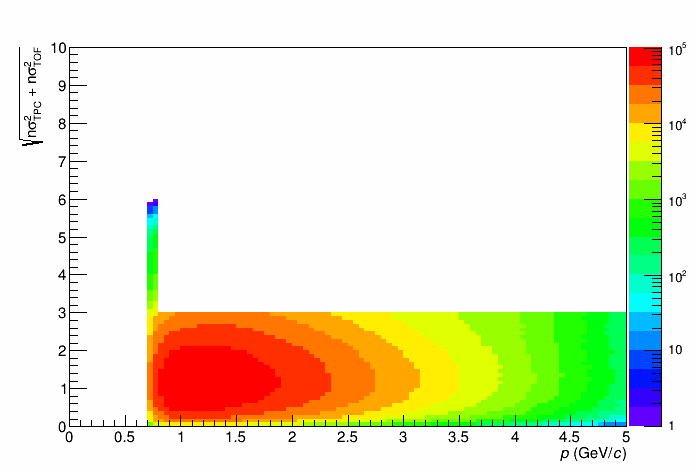
\includegraphics[width=0.32\textwidth]{tpctofnsigma}
   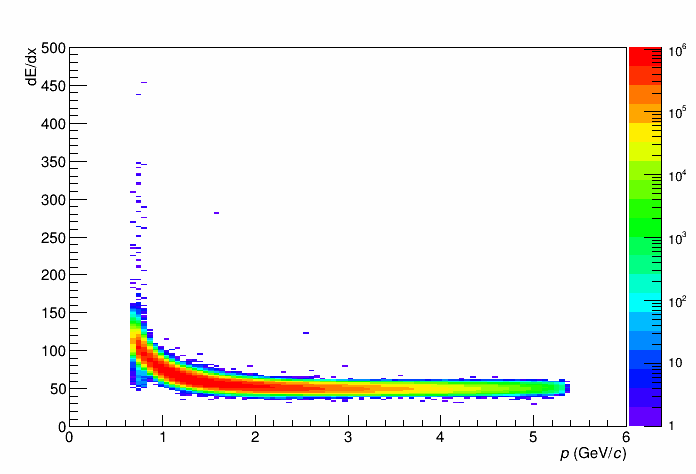
\includegraphics[width=0.32\textwidth]{tpcdedx}
   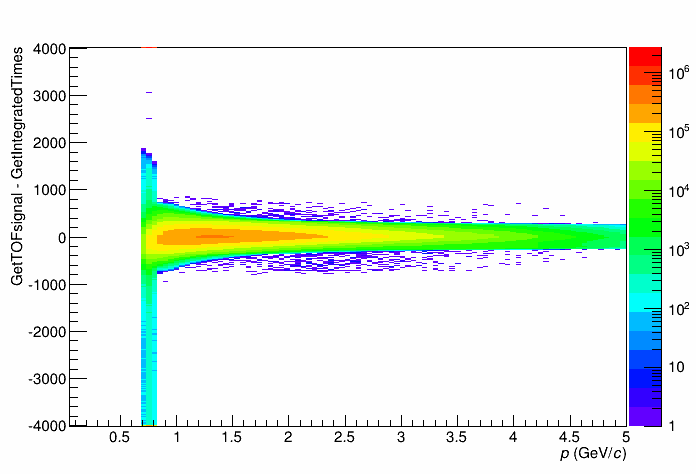
\includegraphics[width=0.32\textwidth]{toftime}
   \caption{Left plot: combined TPC and TOF n$\sigma$ separation vs.  momentum for proton mass hypothesis of accepted tracks. Middle plot: dE/dx signal from TPC. Right plot: signal from TOF.}
   \label{tpctofnsigma}
 \end{figure}

%  \begin{figure}[h!]
%    \centering
%    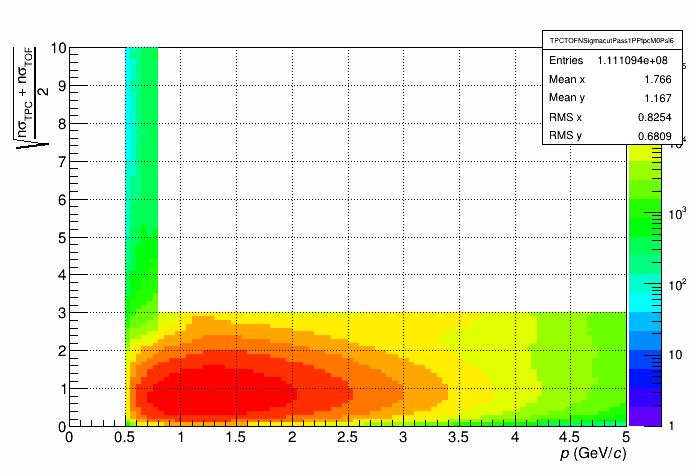
\includegraphics[width=0.49\textwidth]{TPCTOFNsigmaPass_PP}
%    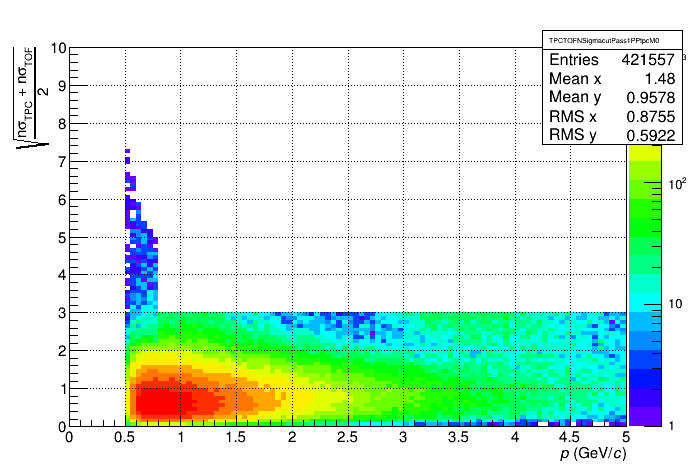
\includegraphics[width=0.49\textwidth]{TPCTOFNsigmaPass_PP_mc}
%    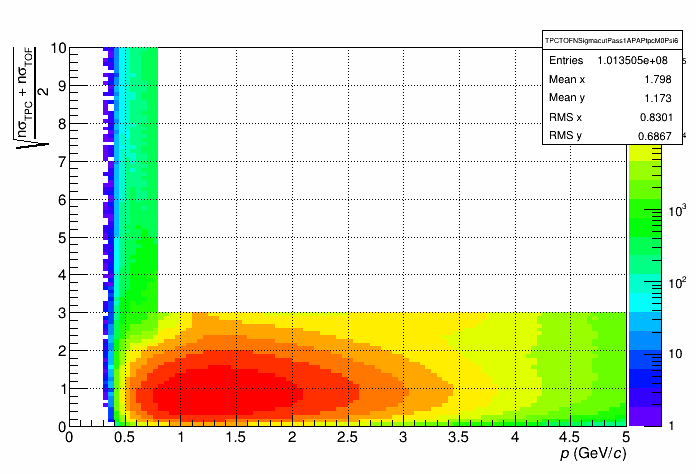
\includegraphics[width=0.49\textwidth]{TPCTOFNsigmaPass_APAP}
%    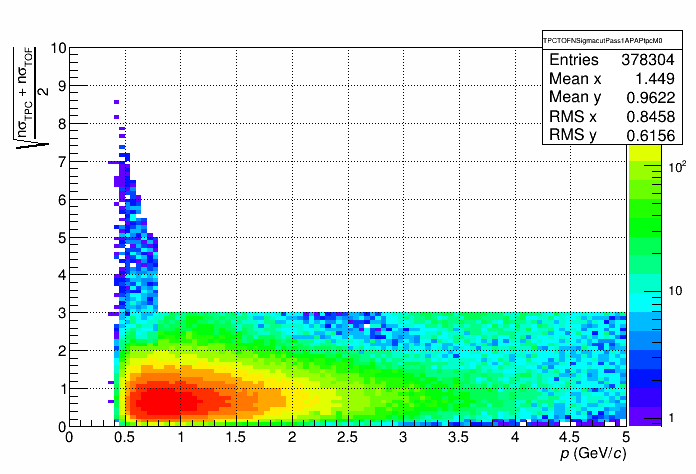
\includegraphics[width=0.49\textwidth]{TPCTOFNsigmaPass_APAP_mc}
%    \caption{Combined TPC and TOF n$\sigma$ separation vs.  momentum for proton mass hypothesis of accepted tracks from data (left plots) and MC (right plots). Top plots refer to protons, bottom plots refer to antiprotons.}
%    \label{tpctofnsigma}
%  \end{figure}
% \begin{figure}[h!]
%   \centering
%   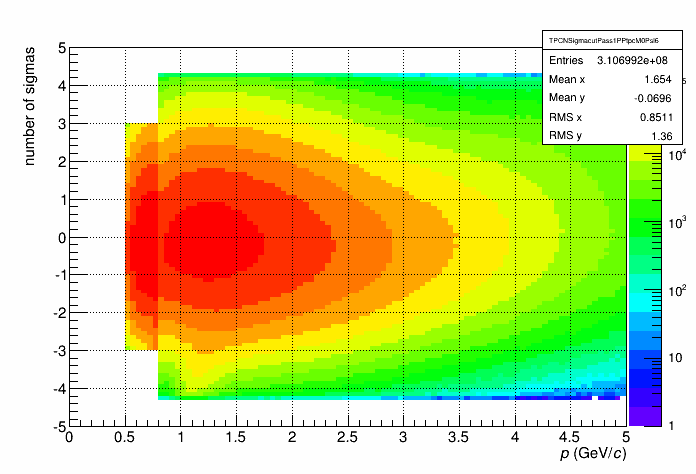
\includegraphics[width=0.49\textwidth]{TPCNsigmaPass_PP}
%   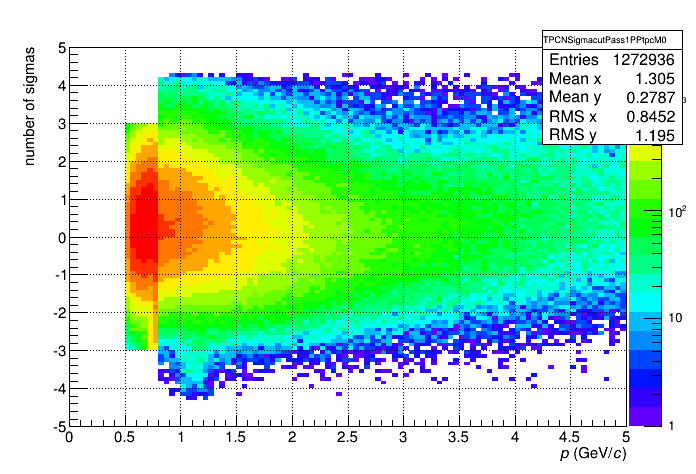
\includegraphics[width=0.49\textwidth]{TPCNsigmaPass_PP_mc}
%   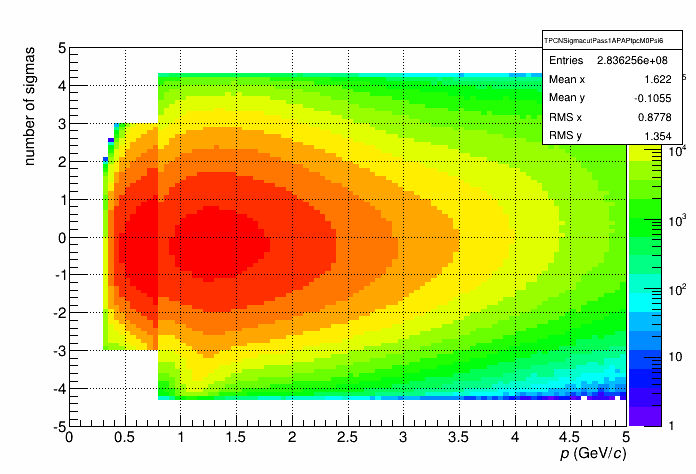
\includegraphics[width=0.49\textwidth]{TPCNsigmaPass_APAP}
%   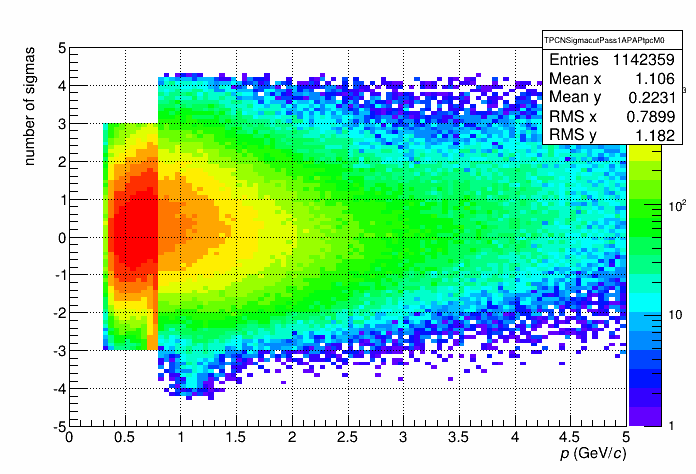
\includegraphics[width=0.49\textwidth]{TPCNsigmaPass_APAP_mc}
%   \caption{TPC n$\sigma$ separation vs.  momentum for proton mass hypothesis of accepted tracks from data (left plots) and MC (right plots). Top plots refer to protons, bottom plots refer to antiprotons.}
%   \label{tpcnsigma}
% \end{figure}
%  \begin{figure}[h!]
%    \centering
%    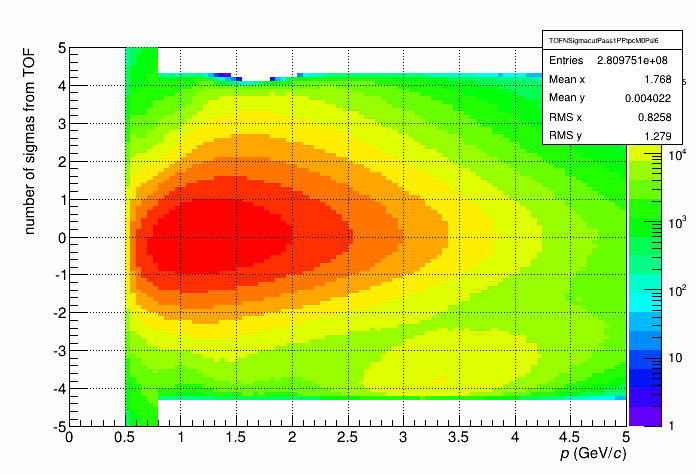
\includegraphics[width=0.49\textwidth]{TOFNsigmaPass_PP}
%    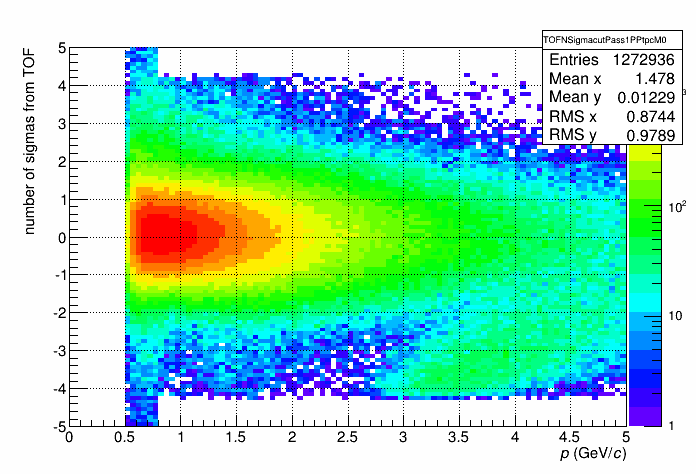
\includegraphics[width=0.49\textwidth]{TOFNsigmaPass_PP_mc}
%    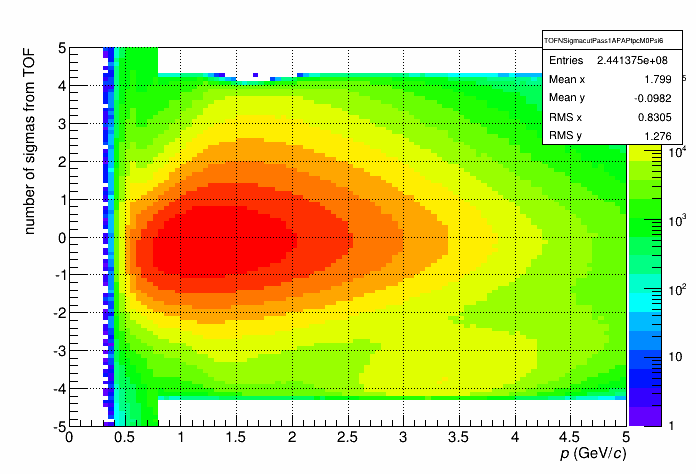
\includegraphics[width=0.49\textwidth]{TOFNsigmaPass_APAP}
%    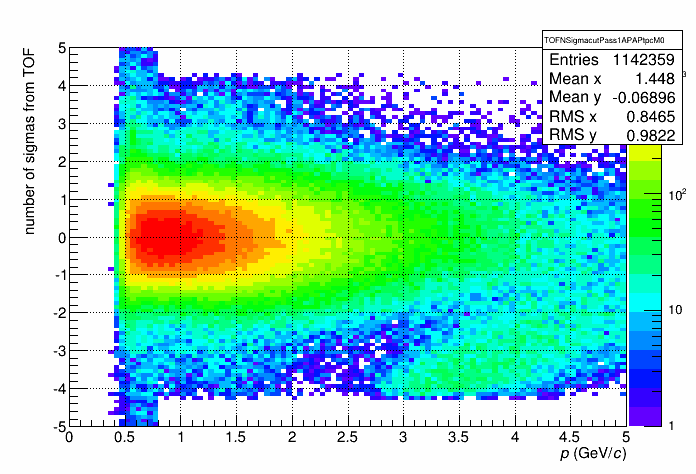
\includegraphics[width=0.49\textwidth]{TOFNsigmaPass_APAP_mc}
%    \caption{TOF n$\sigma$ separation vs. momentum for proton mass hypothesis of accepted tracks from data (left plots) and MC (right plots). Top plots refer to protons, bottom plots refer to antiprotons.}
%    \label{tofnsigma}
%  \end{figure}
% \begin{figure}[h!]
%   \centering
%   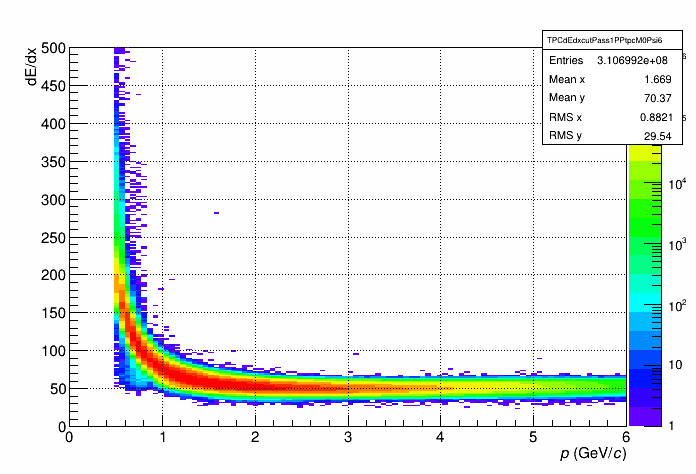
\includegraphics[width=0.49\textwidth]{TPCdEdxPass_PP}
%   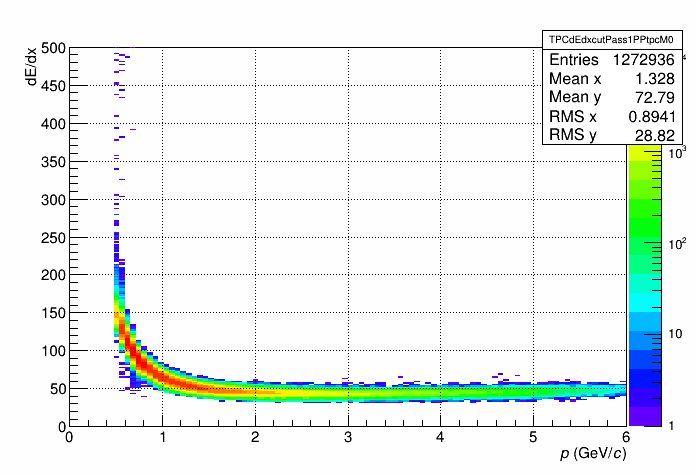
\includegraphics[width=0.49\textwidth]{TPCdEdxPass_PP_mc}
%   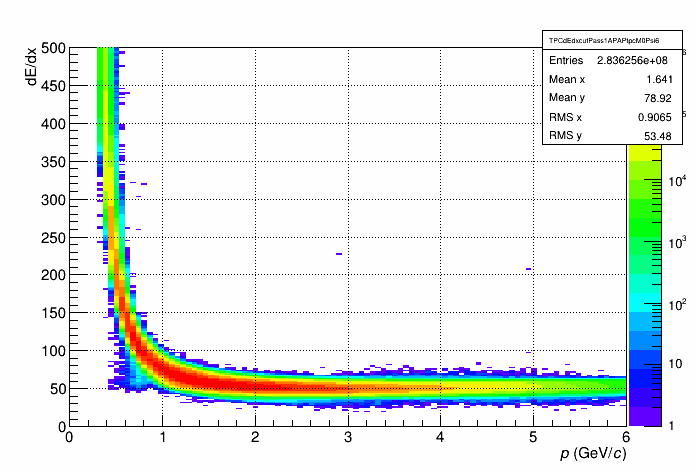
\includegraphics[width=0.49\textwidth]{TPCdEdxPass_APAP}
%   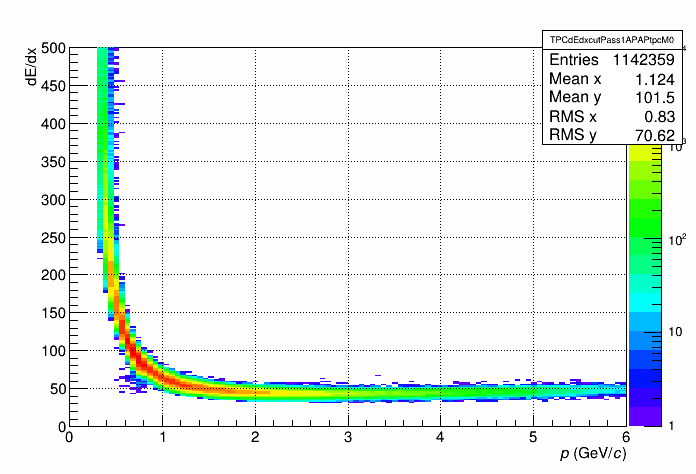
\includegraphics[width=0.49\textwidth]{TPCdEdxPass_APAP_mc}
%   \caption{TPC d$E$/d$x$ vs. momentum for proton mass hypothesis of accepted tracks from data (left plots) and MC (right plots). Top plots refer to protons, bottom plots refer to antiprotons.}
%   \label{tpcnsigma}
% \end{figure}
%  \begin{figure}[h!]
%    \centering
%    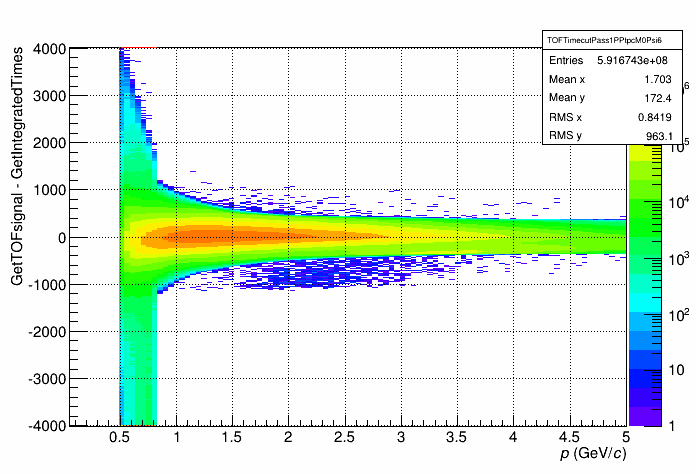
\includegraphics[width=0.49\textwidth]{TOFTimePass_PP}
%    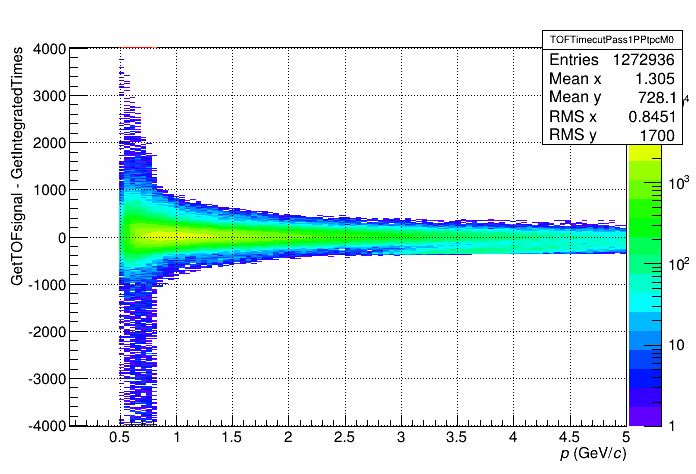
\includegraphics[width=0.49\textwidth]{TOFTimePass_PP_mc}
%    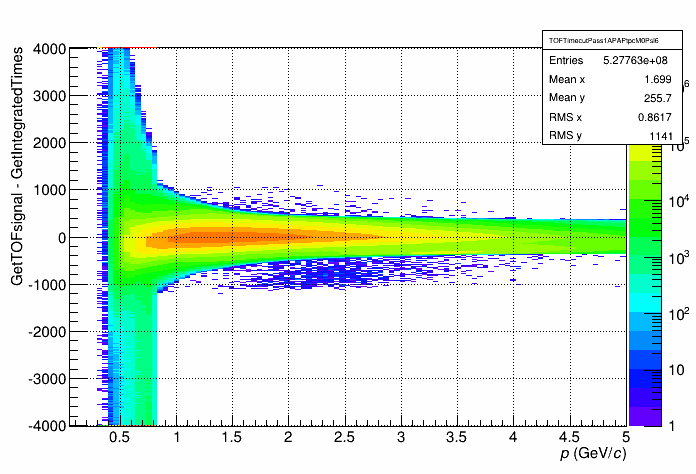
\includegraphics[width=0.49\textwidth]{TOFTimePass_APAP}
%    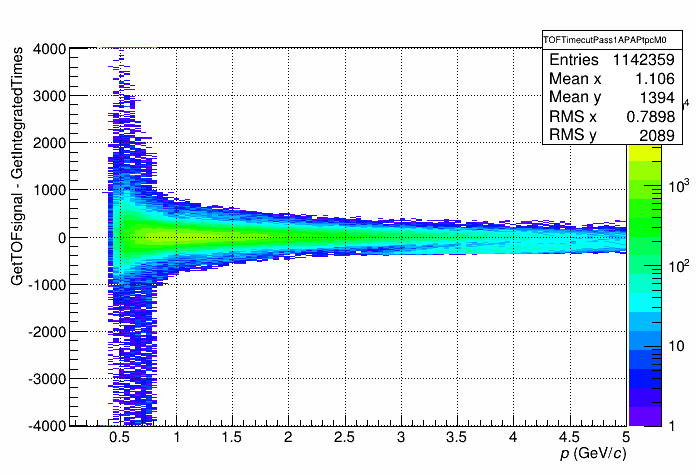
\includegraphics[width=0.49\textwidth]{TOFTimePass_APAP_mc}
%    \caption{TOF time vs. momentum for proton mass hypothesis of accepted tracks from data (left plots) and MC (right plots). Top plots refer to protons, bottom plots refer to antiprotons.}
%    \label{tofnsigma}
%  \end{figure}

% To reduce the contamination from kaons seen in plots from TOF, the alternative method was checked:
% \begin{itemize}
% \item for tracks with $p < 0.8$~GeV/$c$: $n{\sigma}_{TPC} < 3$
% \item for tracks with $0.8 < p < 2.5$~GeV/$c$: ${n{\sigma}_{TPC}} < 3$ and  ${n{\sigma}_{TOF}} < 3$
% \item for tracks with $ p > 2.5$~GeV/$c$: ${n{\sigma}_{TPC}} < 3$ and  ${n{\sigma}_{TOF}} < 2$
% \end{itemize}
% Fig.~\ref{tpctofnsigma2}-\ref{toftime2} show QA of these method of PID.
% \begin{figure}[h!]
%    \centering
%    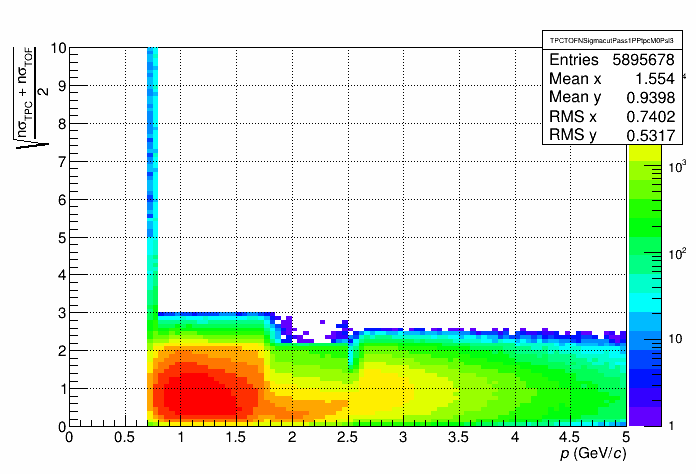
\includegraphics[width=0.49\textwidth]{newpidplots/TPCTOFNsigmaPass_PP}
%    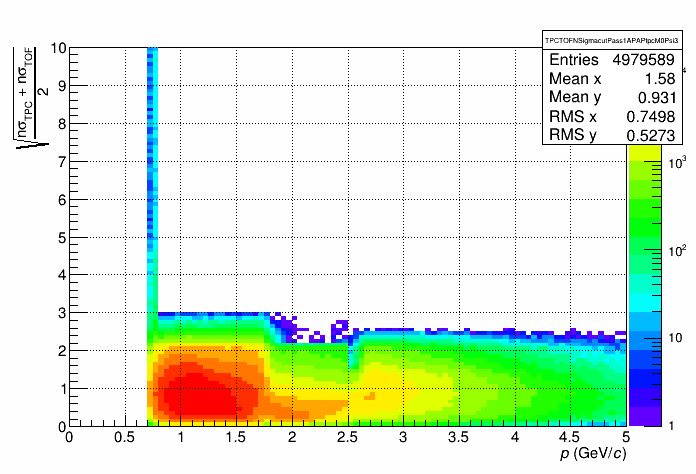
\includegraphics[width=0.49\textwidth]{newpidplots/TPCTOFNsigmaPass_APAP}
%    \caption{Combined TPC and TOF n$\sigma$ separation vs. momentum for proton mass hypothesis of accepted tracks from data. Left plot refer to protons, right plot refer to antiprotons.}
%    \label{tpctofnsigma2}
%  \end{figure}
% \begin{figure}[h!]
%   \centering
%   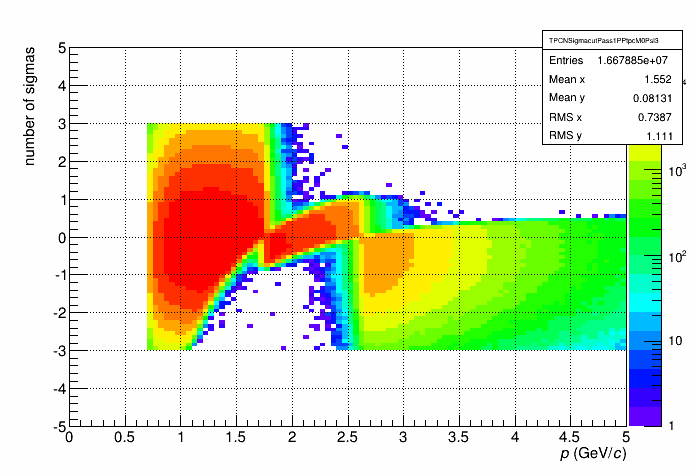
\includegraphics[width=0.49\textwidth]{newpidplots/TPCNsigmaPass_PP}
%   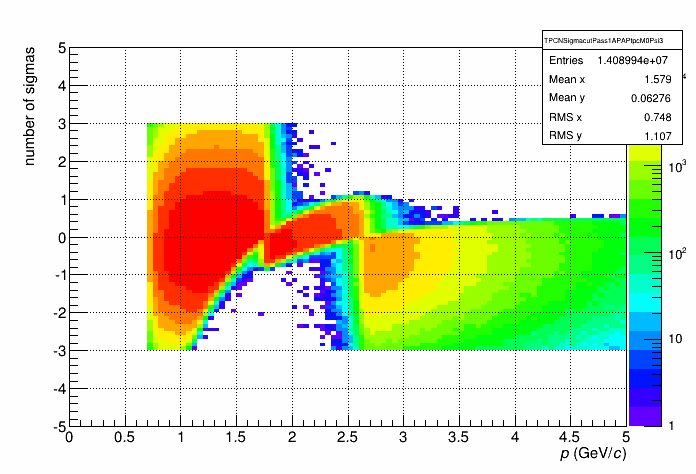
\includegraphics[width=0.49\textwidth]{newpidplots/TPCNsigmaPass_APAP}
%   \caption{TPC n$\sigma$ separation vs.  momentum for proton mass hypothesis of accepted tracks from data. Left plot refer to protons, right plot refer to antiprotons.}
%   \label{tpcnsigma2}
% \end{figure}
%  \begin{figure}[h!]
%    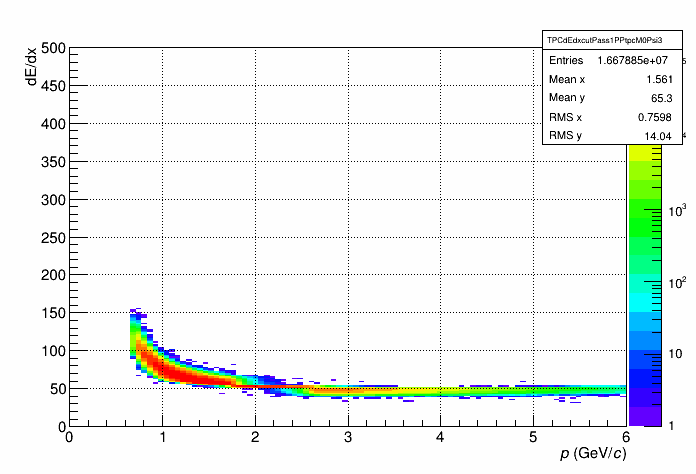
\includegraphics[width=0.49\textwidth]{newpidplots/TPCdEdxPass_PP}
%    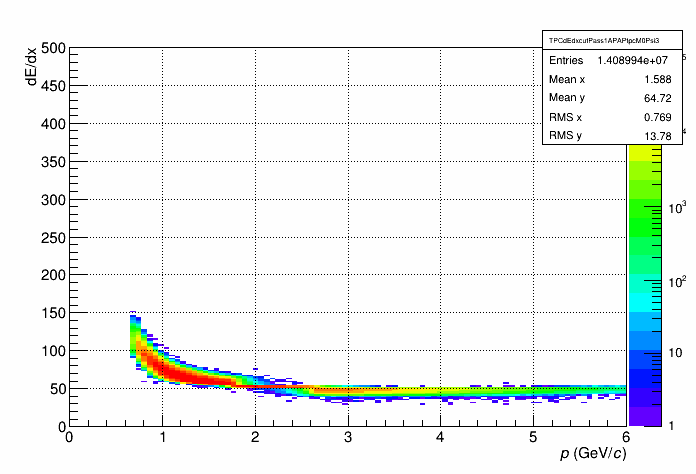
\includegraphics[width=0.49\textwidth]{newpidplots/TPCdEdxPass_APAP}
%    \caption{TPC d$E$/d$x$ vs. momentum for proton mass hypothesis of accepted tracks from data. Left plot refer to protons, right plot refer to antiprotons.}
%    \label{tpcdedx2}
%  \end{figure}
%  \begin{figure}[h!]
%    \centering
%    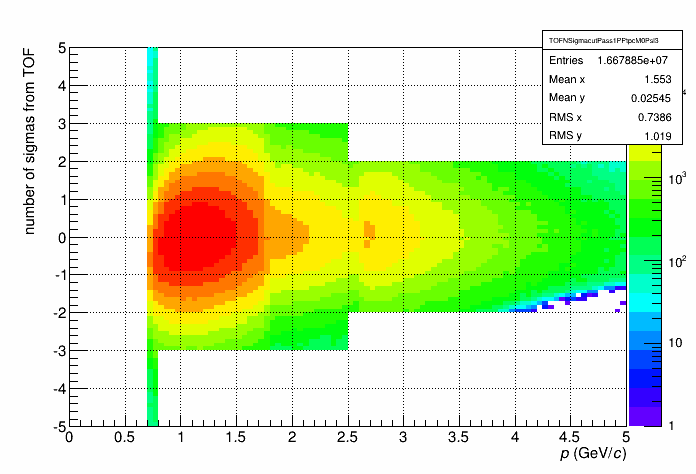
\includegraphics[width=0.49\textwidth]{newpidplots/TOFNsigmaPass_PP}
%    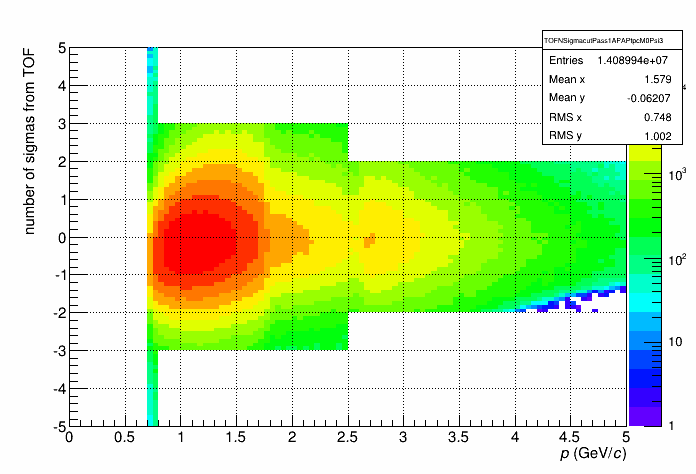
\includegraphics[width=0.49\textwidth]{newpidplots/TOFNsigmaPass_APAP}
%    \caption{TOF n$\sigma$ separation vs. momentum for proton mass hypothesis of accepted tracks from data. Left plot refer to protons, right plot refer to antiprotons.}
%    \label{tofnsigma2}
%  \end{figure}
%  \begin{figure}[h!]
%    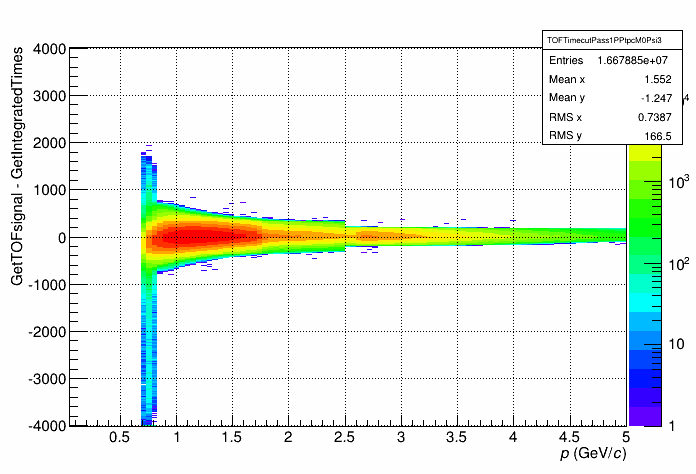
\includegraphics[width=0.49\textwidth]{newpidplots/TOFTimePass_PP}
%    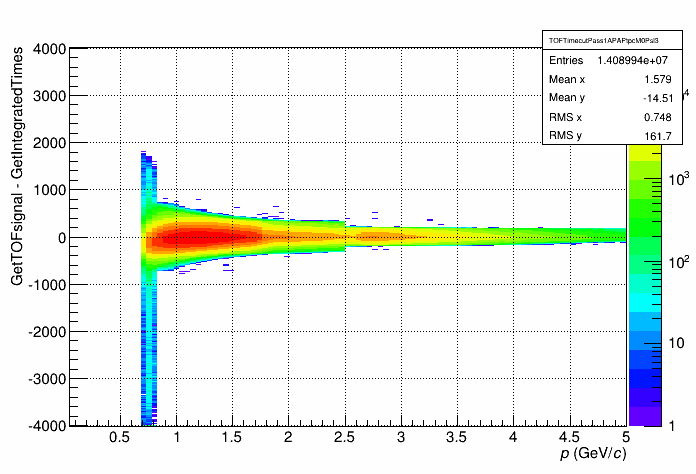
\includegraphics[width=0.49\textwidth]{newpidplots/TOFTimePass_APAP}
%    \caption{TOF time vs. momentum for proton mass hypothesis of accepted tracks from data. Left plot refer to protons, right plot refer to antiprotons.}
%    \label{toftime2}
%  \end{figure}


\subsection{Track selection}
Tracks within the pseudorapidity range $|\eta| < 0.8$ have been selected. We have chosen (anti)protons with $0.7 < p_{\mathrm{T}} < 4.0$~GeV/$c$.
%protons with $0.5 < p_{\mathrm{T}} < 5$~GeV/$c$ and antiprotons with  $0.3 < p_{\mathrm{T}} < 5$~GeV/$c$.
% TODO: protons and antiprotons with 0.7 < pT < 5 GeV/c !!! then pp and apap correlations in first kT bin looks similar
 The minimum number of TPC clusters corresponding to the given track was set to 80 (out of all 159 clusters). The maximum value of $\chi^2$ per TPC cluster was $4.0$ (2 degrees of freedom per cluster). Fig.~\ref{monitors} shows QA plots of the accepted tracks.
\begin{figure}%[h]
  \centering
  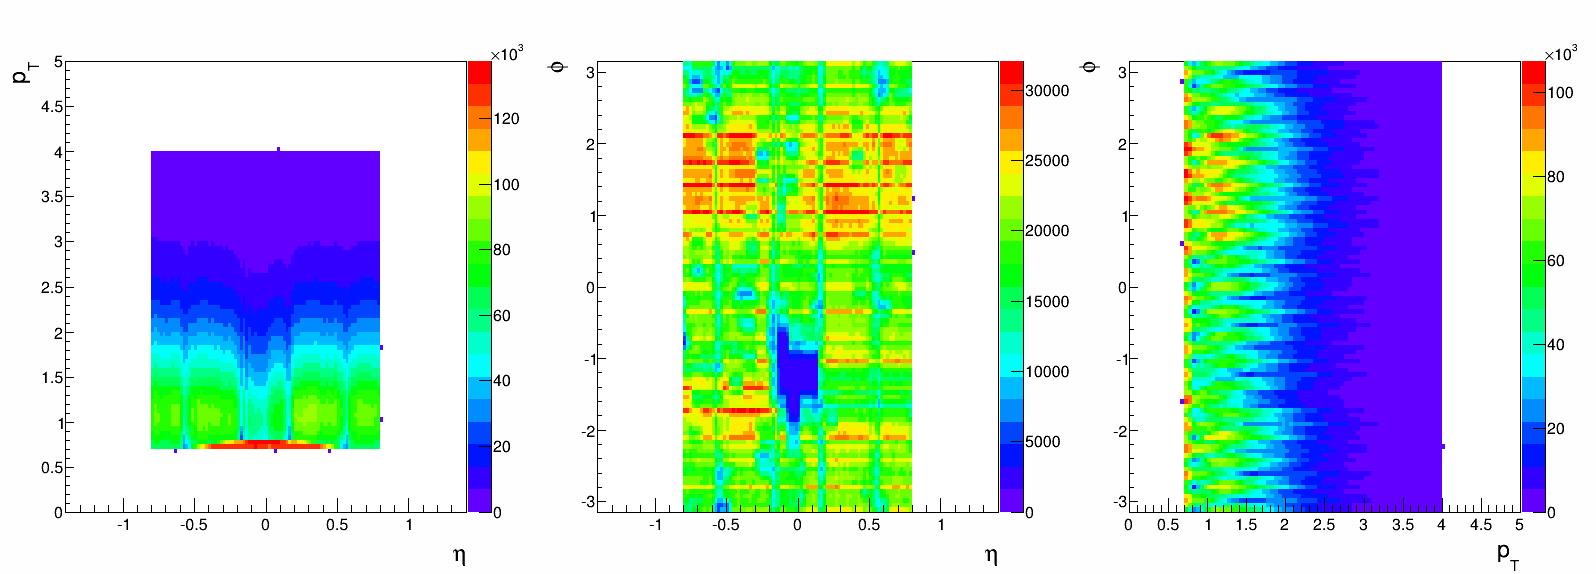
\includegraphics[width=0.9\textwidth]{monitors}
  \caption{QA histograms of accepted tracks.}
  \label{monitors}
\end{figure}

Furthermore, the standard TPC-only track cuts on a Distance of Closest Approach (DCA) was applied: $DCA_{xy} < 2.4 cm$ and  $DCA_{xy} < 3.2 cm$.
In previous studies, to calculate DCA values, we used \verb|PropagateToDCA| method applied for the \emph{global tracks} corresponding to \emph{TPC-only tracks} (similarly as with PID) because of better resolution. The comparison of the DCA distribution in the transverse plane for \emph{TPC-only tracks} and \emph{global tracks} is shown in Fig.~\ref{dca}.
\begin{figure}%[h]
  \centering
  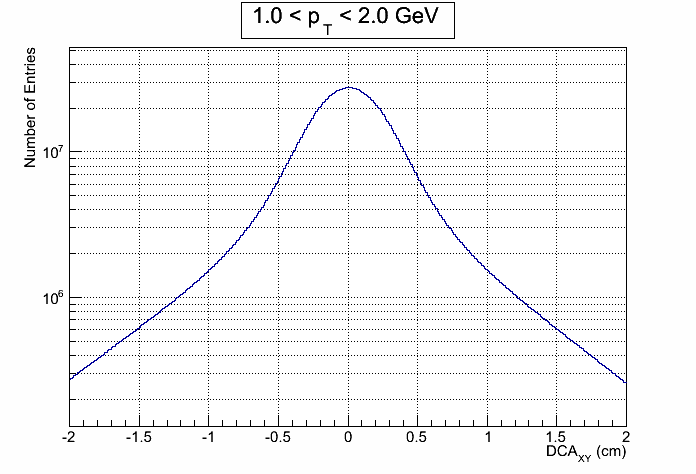
\includegraphics[width=0.49\textwidth]{DCAxyFailProX_PP_tpconly}
  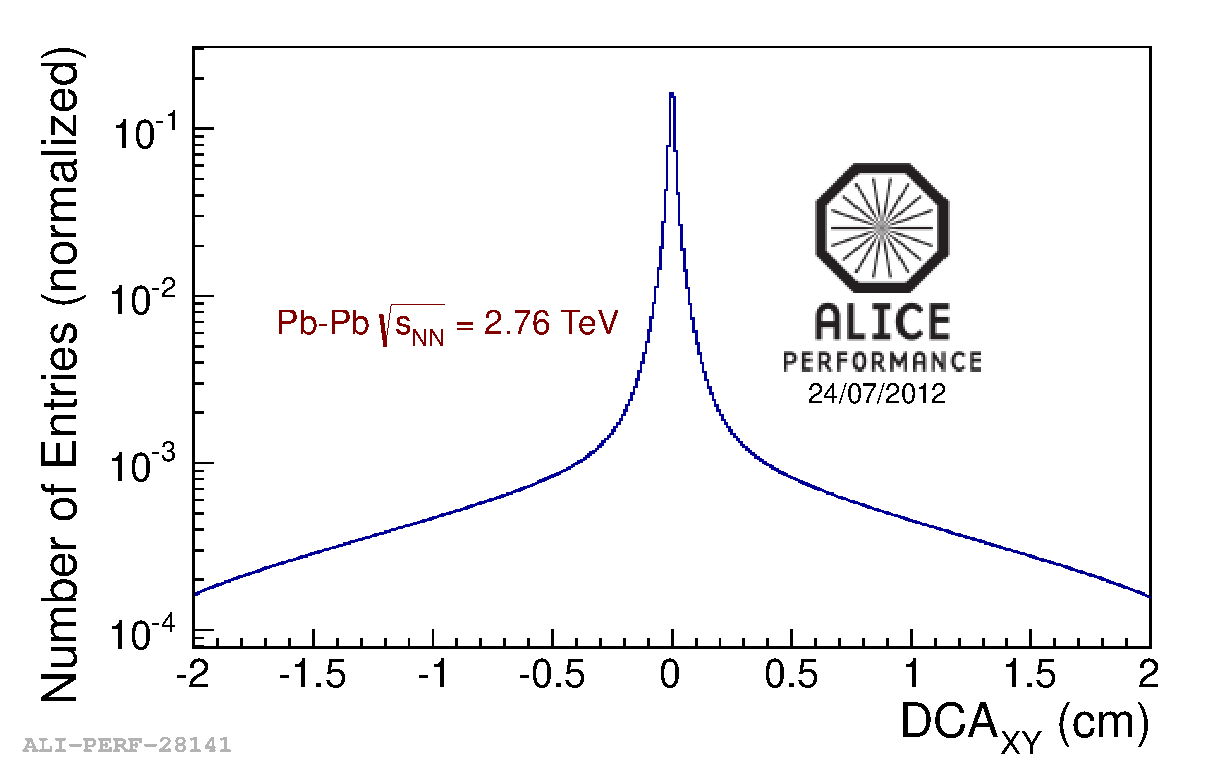
\includegraphics[width=0.49\textwidth]{2012-Jul-25-DCAxyData}
  % 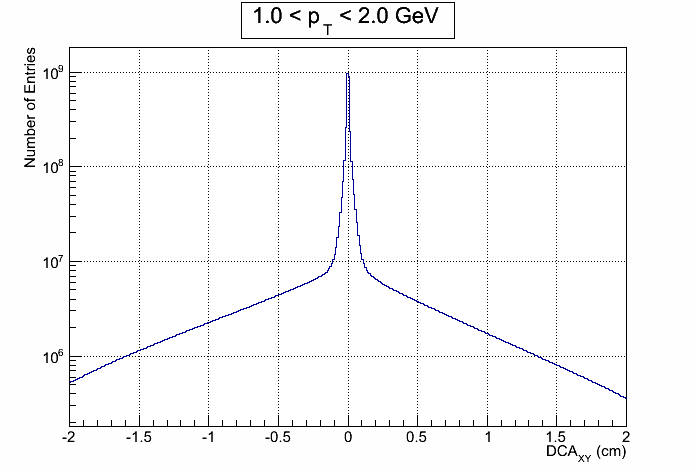
\includegraphics[width=0.49\textwidth]{DCAxyFailProX_PP_global}
  \caption{The comparison of the DCA distribution in the transverse plane for \emph{TPC-only tracks} (left panel) and \emph{global tracks} (right panel).}
  \label{dca}
\end{figure}

However, it caused the unexpected shape of proton-proton correlation functions.

DCA distributions for TPC-only tracks accepted for the analysis are shown in Fig.~\ref{dca}
\begin{figure}%[h]
  \centering
  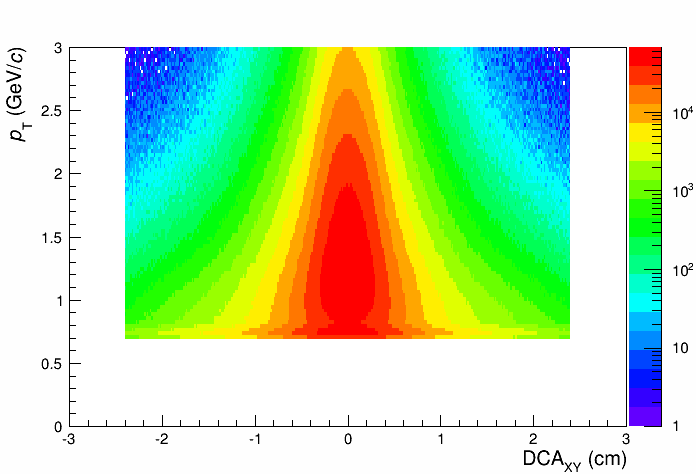
\includegraphics[width=0.49\textwidth]{dcaxy}
  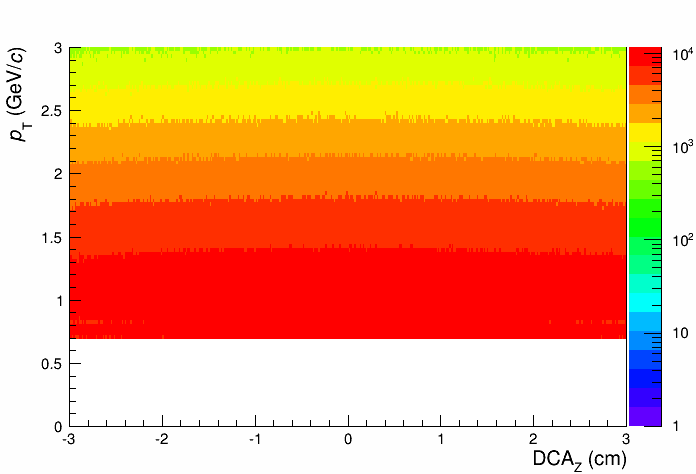
\includegraphics[width=0.49\textwidth]{dcaz}
  \caption{DCA distribution of accepted tracks in the transverse plane (left panel) and in $z$ direction (right panel).}
  \label{dca}
\end{figure}

% Particles located within $2.0$~cm in the beam direction with respect to the primary vertex, were accepted. In the transverse plane, we have used the following cuts:
% \begin{itemize}
% \item $|DCA_{xy}| < 0.1$~cm
% \item $|DCA_{xy}| < 2.4$~cm
% \item $|DCA_{xy}| < 0.018 +0.035 p_{\mathrm T}^{-1.01}$~cm
% \end{itemize}

% The $DCA_{xy}$ distributions in the transverse plane from data are shown in Fig.
%  \begin{figure}%[h]
%    \centering
%    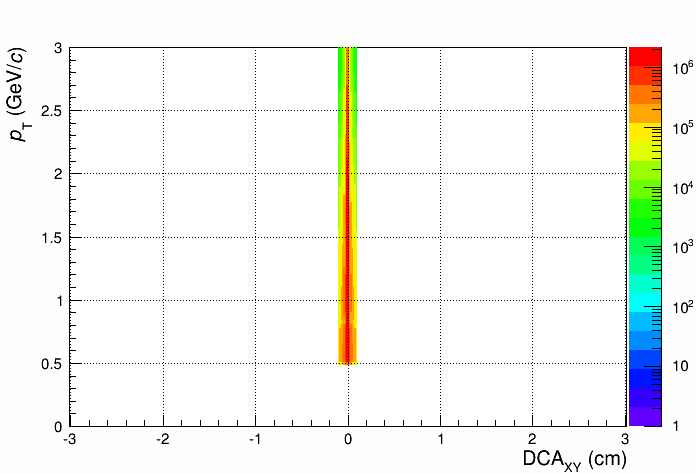
\includegraphics[width=0.49\textwidth]{DCAxyPass_PP_01}
%    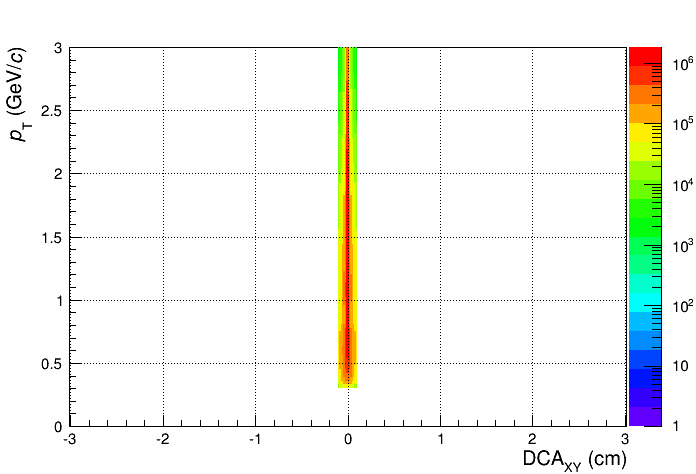
\includegraphics[width=0.49\textwidth]{DCAxyPass_APAP_01}
%    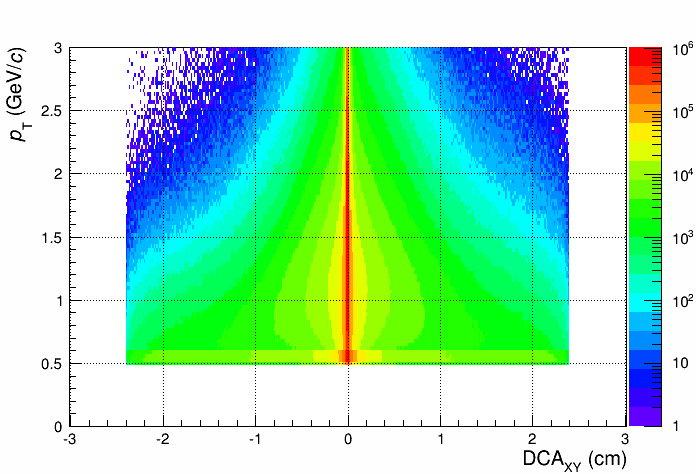
\includegraphics[width=0.49\textwidth]{DCAxyPass_PP_24}
%    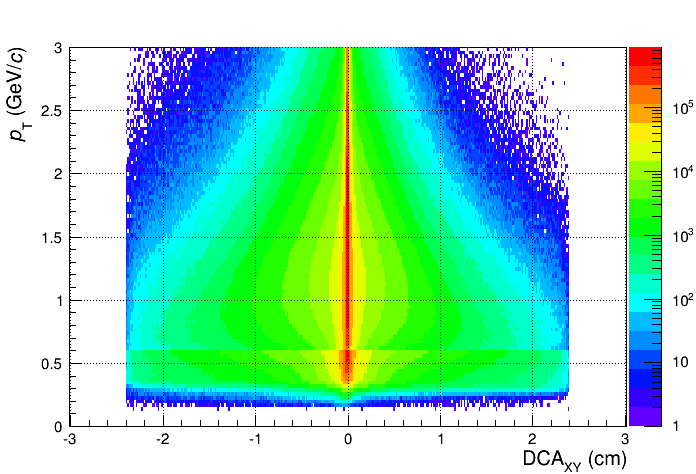
\includegraphics[width=0.49\textwidth]{DCAxyPass_APAP_24}
%    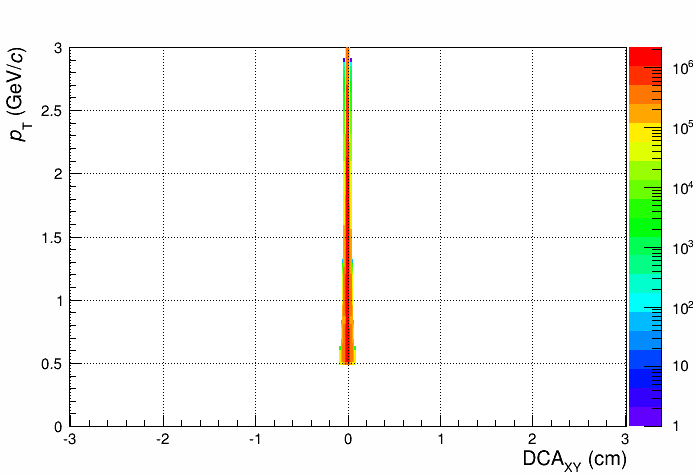
\includegraphics[width=0.49\textwidth]{DCAxyPass_PP_ptdep}
%    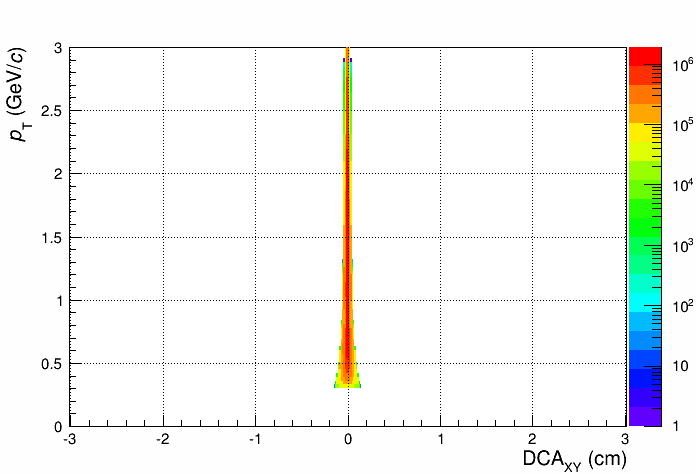
\includegraphics[width=0.49\textwidth]{DCAxyPass_APAP_ptdep}
%    \caption{The $DCA_{xy}$ distributions  for different cut values (listed above, in the text) from top to bottom for protons (left plots) and antiprotons (right plots).}
%    \label{tofnsigma}
%  \end{figure}

The contamination from secondary particles ((anti)protons from weak decays and protons produced by interactions of particles with detector material) was estimated using MC (HIJING, LHC11a10a\_bis, AOD120). It was done using DCA information from global tracks corresponding to TPC-only tracks. Fig.~\ref{dcatemplates} shows $DCA_{xy}$ template distributions of protons and antiprotons: for primary particles, particles from weak decays and particles from material (there was also non-zero fraction of antiprotons ``from material'', but they are not shown and were excluded from the fitting procedure).
 \begin{figure}%[h]
   \centering
   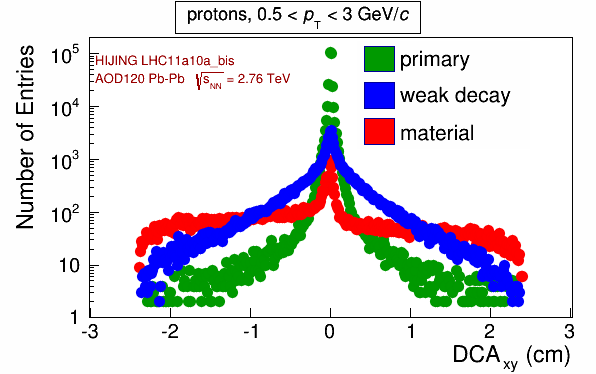
\includegraphics[width=0.49\textwidth]{DCAxyMC_hijing_PP}
   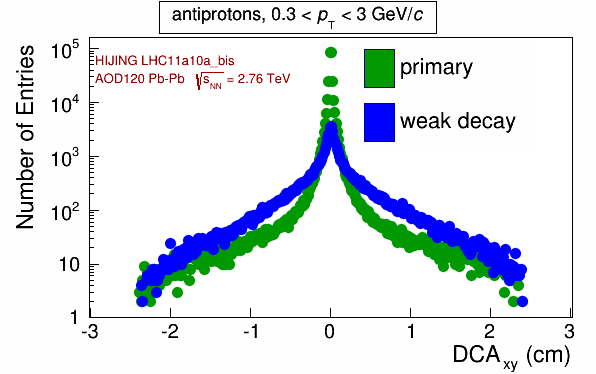
\includegraphics[width=0.49\textwidth]{DCAxyMC_hijing_APAP}
   \caption{The $DCA_{xy}$ (for global tracks) template distributions of protons (left plot) and antiprotons (right plot) with respect to theirs origin.}
   \label{dcatemplates}
 \end{figure}
Templates obtained for TPC-only tracks are shown in Fig.~\ref{dcatemplatestpconly}. Similar shapes of all contribution make the relaible fitting impossible.
 \begin{figure}%[h]
   \centering
   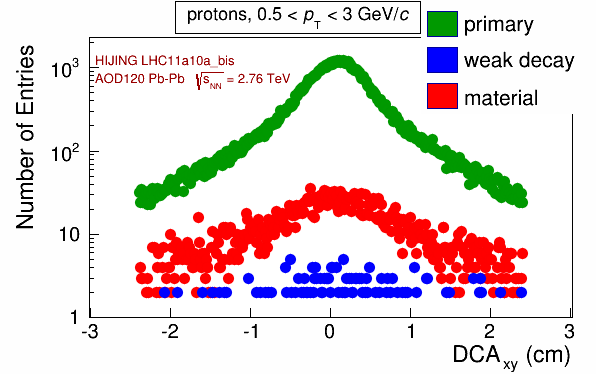
\includegraphics[width=0.49\textwidth]{DCA_MCtemplates_tpconly}
   \caption{The $DCA_{xy}$ (for TPC-only tracks) template distributions of protons with respect to theirs origin.}
   \label{dcatemplatestpconly}
 \end{figure}

To calculate the relative contribution of each source of contamination, the data distribution is fitted in [-2.4;2.4]cm range with the template distributions in $p_{\mathrm T}$ bins (10 for protons, 11 for antiprotons). The fit was done using TFractionFitter class from ROOT. Examples of fits are shown in Fig.~\ref{fittemplate}.
 \begin{figure}%[h]
   \centering
   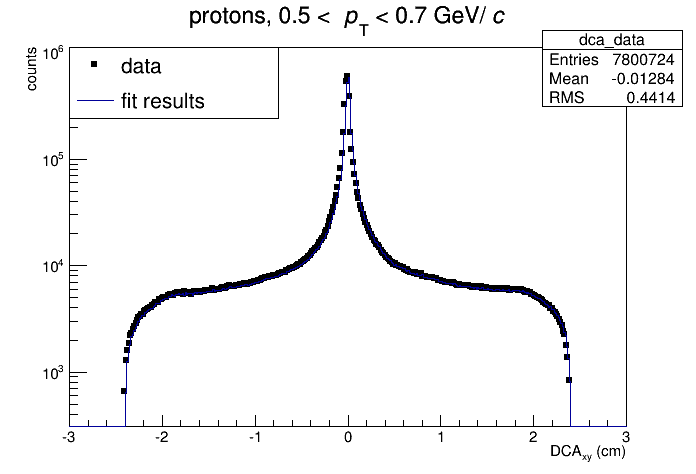
\includegraphics[width=0.49\textwidth]{dcafitPP}
   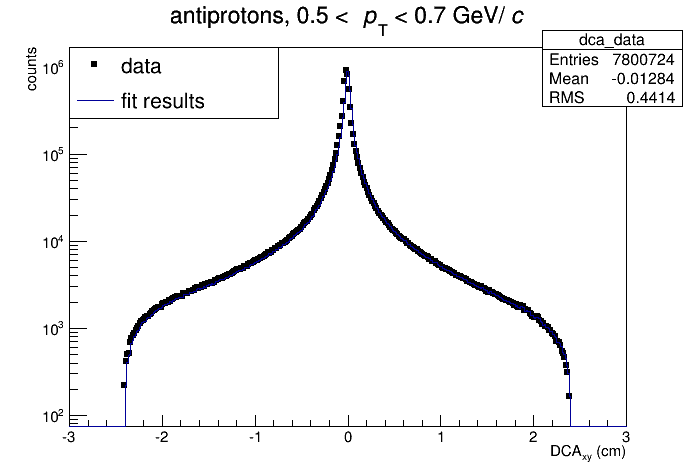
\includegraphics[width=0.49\textwidth]{dcafitAPAP}
   \caption{Examples of fit of $DCA_{xy}$  distributions with MC templates.}
   \label{fittemplate}
 \end{figure}

Results of the fits are shown in Fig.~\ref{fractions}.
 \begin{figure}%[h]
   \centering
   \includegraphics[width=0.89\textwidth]{fractions}
   \caption{Fractions of (anti)protons with respect to theirs origin obtained from MC template fits.}
   \label{fractions}
 \end{figure}


%% The cut value $0{.}1$~cm was determined using MC simulations to obtain the highest significance. %Purity of protons was estimated as $80\%$ and $90\%$ and of antiprotons as $84\%$ and $92\%$ in AMPT and HIJING, respectively.
%% Purity of (anti)protons estimated in MC (HIJING and AMPT) simulations is shown in Tab.~\ref{fractions}. The DCA distribution of protons with respect to its origin from MC simulation (AMPT) is shown in Fig.~\ref{dcatemplates}.
%% \begin{table}[h]
%%   \begin{tabularx}{\textwidth}{|X|X|X|X|X|} \hline
%%     % \centering
%%     % \textbf{B} & \textbf{Centr.} & \boldmath{$17{.}3 \unit{GeV}$} & \boldmath{$27 \unit{GeV}$} & \boldmath{$39 \unit{GeV}$} \\ \hline
%%     \centering
%%     & \multicolumn{2}{|c|}{HIJING} & \multicolumn{2}{|c|}{AMPT}   \\ \cline{2-5}
%%     \centering
%%     &   p &   $\bar{\mathrm{p}}$  &  p &  $\bar{\mathrm{p}}$ \\ \hline
%%     \centering
%%     primary &  $91\%$ & $90\%$  & $88\%$ & $80\%$ \\ \hline
%%     \centering
%%     weak decays & $8\%$ & $9\%$  & $11\%$ & $20\%$ \\ \hline
%%     \centering
%%     material & $1\%$ & $1\%$  & $1\%$ & $0\%$ \\ \hline

%%   \end{tabularx}
%%   \caption{Fractions of (anti)protons with respect to its origin from MC simulations.}
%%   \label{fractions}
%% \end{table}
% \begin{table}[h]
%   \begin{tabularx}{\textwidth}{|X|X|X|X|X|} \hline
%     % \centering
%     % \textbf{B} & \textbf{Centr.} & \boldmath{$17{.}3 \unit{GeV}$} & \boldmath{$27 \unit{GeV}$} & \boldmath{$39 \unit{GeV}$} \\ \hline
%     \centering
%     & \multicolumn{2}{|c|}{HIJING} & \multicolumn{2}{|c|}{AMPT}   \\ \cline{2-5}
%     \centering
%     &   p &   $\bar{\mathrm{p}}$  &  p &  $\bar{\mathrm{p}}$ \\ \hline
%     \centering
%     primary &  $53\%$ & $85\%$  & $57\%$ & $75\%$ \\ \hline
%     \centering
%     $\Lambda$ ($\bar{\Lambda}$) decay & $6\%$ & $11\%$  & $9\%$ & $17\%$ \\ \hline
%     \centering
%     $\Sigma^+$ ($\bar{\Sigma^+}$) decay & $2\%$ & $2\%$  & $3\%$ & $7\%$ \\ \hline
%     \centering
%     rest & $39\%$ & $2\%$  & $31\%$ & $1\%$ \\ \hline

%   \end{tabularx}
%   \caption{Fractions of (anti)protons with respect to its origin from MC simulations.}
%   \label{fractions}
% \end{table}

%% \begin{figure}%[h]
%%   \centering
%%   \includegraphics[width=0.7\textwidth]{2012-Jul-25-DCAxyMC}
%%   \caption{The DCA distribution of protons with respect to its origin from MC simulation (AMPT).}
%%   \label{dcatemplates}
%% \end{figure}


\subsection{Pair selection}
In case of pair selection criteria, standard cuts preventing the effects of merging (two tracks reconstructed as one) and splitting (one track reconstructed as two) were used. Strictly speaking, the cuts consists of two steps: \emph{share quality} and \emph{share fraction}. The former one bases on the calculation of the fraction of the number of clusters on the same TPC pad row shared by both tracks to the number of all clusters of the two tracks. Maximum \emph{share quality} was set to $1.0$ which means accepting all pairs. As regards \emph{share fraction}, it is obtained as a ratio of shared clusters to all clusters of both tracks. All pairs sharing more than $5 \%$ clusters were rejected.
The cut on angular distance~\cite{phistar} have been applied. Fig.~\ref{cfpphijingnophi} shows proton-proton correlation function from HIJING before and after applying the cut.
\begin{figure}%[h]
  \centering
  \includegraphics[width=0.9\textwidth]{cfpphijing}
  \caption{pp correlation function from HIJING simulations without the cut on angular distance (left panel) and with the cut $|\Delta\varphi^*_{@R=1.2m}| < 0.045$, $|\Delta\eta| < 0.01$ (right panel).}
  \label{cfpphijingnophi}
\end{figure}
% Pairs separated in the angular distance less than $0.018$~rad in $\varphi^*$ (modified azimuthal angle taking into account bending inside the magnetic field) and less than $0.015$ in $\eta$ at the radius within TPC $1.1$~m will be rejected. Due to the necessity of the knowledge of magnetic field polarity, the analysis need to be performed for \emph{field~$--$} and \emph{field~$++$} runs separately.
Only pairs within  $|\Delta\varphi^*_{@R=1.2m}| < 0.045$, $|\Delta\eta| < 0.011$) are accepted.  Angular distance $|\Delta\varphi^*| = \varphi_1 - \varphi_2 + \arcsin(\frac{e B R}{2 p_{T1}}) - \arcsin(\frac{e B R}{2 p_{T1}})$, where $\varphi$ - azimuthal angle of the track at the vertex, $e$ - elementary charge (-0.3 in Heaviside-Lorentz units), $B$ - magnetic field, $R$ - radius in TPC, $p_T$ - transverse momentum ,  is calculated for TPC radius $R = 1.2~m$.
%\frac{z \cdot e \cdot B \cdot R}{2 p_T_1})$

% In Fig.\ref{phistaretahijing} $\Delta \varphi^* \Delta \eta$ distribution from HIJING simulations is shown.
% \begin{figure}%[h]
%   \centering
%   \includegraphics[width=0.9\textwidth]{phistaretahijing}
%   \caption{$\Delta \varphi^* \Delta \eta$ distribution from HIJING simulations.}
%   \label{phistaretahijing}
% \end{figure}
% Due to the necessity of the knowledge of magnetic field polarity, the analysis need to be performed for \emph{field~$--$} and \emph{field~$++$} runs separately. However, obtained correlation functions are consistent, so we use all runs together, to have bigger statistics.

\subsection{Correlation functions}

Two-particle correlations were studied in one dimensional representation with respect to the relative momentum  $q_{\mathrm{inv}}=2 \cdot k^{*} = \sqrt{(p_1-p_2)^2-(E_1-E_2)^2}$. The correlation effect was measured with the function defined as:
\begin{equation}
  C(q_{\mathrm{inv}}) = \frac{A(q_{\mathrm{inv}})}{B(q_{\mathrm{inv}})},
\end{equation}
where $A(q_{\mathrm{inv}})$ is a distribution of correlated pairs of particles (coming from the same event), $B(q_{\mathrm{inv}})$ is a distribution of uncorrelated pairs of particles (coming from different events - 10 events were used to create the background distribution).

%TODO: write about binning in event plane angle to reduce non-flat background
%TODO: fit with the baseline parametrized by some function like in pPb and pp
%TODO: look at different number of psi bins and compare (3 vs 6 vs 12)
%TODO: fitting in psi bins

The analysis has been performed for six centrality bins ($0-5\%$, $5-10\%$, $10-20\%$, $20-30\%$, $30-40\%$, $40-50\%$) and then merged into three classes: $0-10\%$,~$10-30\%$ and $30-50\%$. Also, correlation functions have been calculated for two bins of the pair transverse momentum $k_{\mathrm{T}}~=~(|\vec{p}_{\mathrm{T,1}}+\vec{p}_{\mathrm{T,2}}|)/2$: $0.01<k_{\mathrm{T}}<1{.}00$~GeV/$c$ and $1 < k_{\mathrm{T}}<5$~GeV/$c$.

\section{Results}

\subsection{Investigation of non-flat background of correlation function at large $q$}
In Fig.~\ref{nonflat} and~\ref{nonflatmc} one can observe that pp, $\bar{\mathrm{p}}\bar{\mathrm{p}}$ and p$\bar{\mathrm{p}}$ correlation functions at large $q$ deviate from unity. The effect increases with centrality and $k_{\mathrm T}$. The effect is qualitatively similar for p$\bar{\mathrm{p}}$ correlations in MC simulations, despite HIJING at low $k_{\mathrm T}$.

\begin{figure}%[h!]
  \centering
  \includegraphics[width=0.49\textwidth]{papnf}
  \includegraphics[width=0.49\textwidth]{papnf2}
  \includegraphics[width=0.49\textwidth]{apapnf}
  \includegraphics[width=0.49\textwidth]{apapnf2}
  \caption{Proton-antiproton and antiproton-antiproton correlation functions for the $\sqrt{s_{\mathrm{NN}}}=2.76$~TeV Pb--Pb in wide $q$ range.}
  \label{nonflat}
\end{figure}

\begin{figure}%[h!]
  \centering
  \includegraphics[width=0.49\textwidth]{papnfampt}
  \includegraphics[width=0.49\textwidth]{papnf2ampt}
  \includegraphics[width=0.49\textwidth]{papnfhijing}
  \includegraphics[width=0.49\textwidth]{papnf2hijing}
  \caption{Proton-antiproton correlation functions for the AMPT and HIJING $\sqrt{s_{\mathrm{NN}}}=2.76$~TeV Pb--Pb in wide $q$ range.}
  \label{nonflatmc}
\end{figure}

The analysis was redone calculating numerators and denominators in bins of the event plane angle from VZERO detector (\verb|GetEventplane| method from \verb|AliEventplane| class). To study the effect of mixing in event plane angle bins on the shape of correlation function at large $q$, two methods are compared:
\begin{itemize}
\item without EP angle selection
  \begin{itemize}
  \item numerators and denominators from each run added
  \item summed numerator divided by summed denominator
  \item correlation function scaled by \\ \verb|den->GetEntries()/num->GetEntries()|
  \end{itemize}
\item calculations in 6 EP bins, then:
  \begin{itemize}
  \item numerators from each run and $\Psi_2$ bin added
  \item denominators from each run and $\Psi_2$ bin scaled by \\ \verb|num[run][psi]->GetEntries()/den[run][psi]->GetEntries()| and then added
  \item correlation function: numerator divided by denominator
  \end{itemize}
\end{itemize}
Results with 6 event plane angle bins are shown in Fig.~\ref{pappsi}, Fig.~\ref{pppsi}, Fig.~\ref{apappsi}. One can notice that the background is slightly more flat in the method with event plane angle binning. However, the effect is rather small, especially for identical pairs.

\begin{figure}%[h!]
  \centering
  \includegraphics[width=0.99\textwidth]{pappsi}
  \caption{Comparison proton-antiproton of correlation functions calculated without and with 6 event plane angle selection.}
  \label{pappsi}
\end{figure}
\begin{figure}%[h!]
  \centering
  \includegraphics[width=0.99\textwidth]{pppsi}
  \caption{Comparison of proton-proton correlation functions calculated without and with 6 event plane angle selection.}
  \label{pppsi}
\end{figure}
\begin{figure}%[h!]
  \centering
  \includegraphics[width=0.99\textwidth]{apappsi}
  \caption{Comparison of antiproton-antiproton correlation functions calculated without and with 6 event plane angle selection.}
  \label{apappsi}
\end{figure}

Results with 3 event plane angle bins are shown in Fig.~\ref{pappsi3}, Fig.~\ref{pppsi3}, Fig.~\ref{apappsi3}. The difference between two methods is much smaller compared to 6-bins case.
\begin{figure}%[h!]
  \centering
  \includegraphics[width=0.49\textwidth]{cfPAPsemicentral_ptdcattcpsipidkT0c2}
  \includegraphics[width=0.49\textwidth]{cfPAPsemicentral_ptdcattcpsipidkT0c4}
  \includegraphics[width=0.49\textwidth]{cfPAPsemicentral_ptdcattcpsipidkT1c2}
  \includegraphics[width=0.49\textwidth]{cfPAPsemicentral_ptdcattcpsipidkT1c4}
  \caption{Comparison of proton-antiproton of correlation functions calculated without and with 3 event plane angle selection. Top plots: $\langle k_T \rangle = 0.6 GeV/c$, bottom plots: $\langle k_T \rangle = 1.5 GeV/c$, left plots: $10-30 \%$, right plots: $30-50 \%$}
  \label{pappsi3}
\end{figure}
\begin{figure}%[h!]
  \centering
  \includegraphics[width=0.49\textwidth]{cfPPsemicentral_ptdcattcpsipidkT0c2}
  \includegraphics[width=0.49\textwidth]{cfPPsemicentral_ptdcattcpsipidkT0c4}
  \includegraphics[width=0.49\textwidth]{cfPPsemicentral_ptdcattcpsipidkT1c2}
  \includegraphics[width=0.49\textwidth]{cfPPsemicentral_ptdcattcpsipidkT1c4}
  \caption{Comparison of proton-proton of correlation functions calculated without and with 3 event plane angle selection. Top plots: $\langle k_T \rangle = 0.6 GeV/c$, bottom plots: $\langle k_T \rangle = 1.5 GeV/c$, left plots: $10-30 \%$, right plots: $30-50 \%$}
  \label{pppsi3}
\end{figure}
\begin{figure}%[h!]
  \centering
  \includegraphics[width=0.49\textwidth]{cfAPAPsemicentral_ptdcattcpsipidkT0c2}
  \includegraphics[width=0.49\textwidth]{cfAPAPsemicentral_ptdcattcpsipidkT0c4}
  \includegraphics[width=0.49\textwidth]{cfAPAPsemicentral_ptdcattcpsipidkT1c2}
  \includegraphics[width=0.49\textwidth]{cfAPAPsemicentral_ptdcattcpsipidkT1c4}
  \caption{Comparison of antiproton-antiproton of correlation functions calculated without and with 3 event plane angle selection. Top plots: $\langle k_T \rangle = 0.6 GeV/c$, bottom plots: $\langle k_T \rangle = 1.5 GeV/c$, left plots: $10-30 \%$, right plots: $30-50 \%$}
  \label{apappsi3}
\end{figure}

Results with 12 event plane angle bins are shown in Fig.~\ref{psi12}. The difference between two methods is also smaller compared to 6-bins case.
\clearpage
\begin{figure}%[h!]
  \centering
  \includegraphics[width=0.49\textwidth]{pap_12psibins_3050_kt1.png}
  \includegraphics[width=0.49\textwidth]{pp_12psibins_3050_kt1.png}
  \caption{Comparison of proton-antiproton (left plot) and proton-proton (right plot) correlation functions calculated without and with 12 event plane angle selection ($\langle k_T \rangle = 1.5 GeV/c$, centrality$30-50 \%$})
  \label{psi12}
\end{figure}

Due to high memory cost of the method with binning in event plane angle, all subsequent results were obtained using standard method, without event plane angle selection. It is justified as there are no significant differences on the low-q region, which contains femtoscopic information and plays a key role in fitting.

\subsection{Correlation functions}
\label{sec:results}

Correlation functions were calculated with different sets of cuts which are summarized in Tab.~\ref{cuts}
\begin{table}[h]
  \begin{tabularx}{\textwidth}{|X|c|c|c|c|c|} \hline
    \centering
    % & \multicolumn{4}{|c|}{R (fm)}    \\ \hline
    % & \multicolumn{1}{|c|}{pp} & \multicolumn{2}{|c|}{ $\bar{\mathrm{p}}$ $\bar{\mathrm{p}}$} & \multicolumn{1}{|c|}{p$\bar{\mathrm{p}}$}   \\ \hline
    \centering
     &   $p_T (GeV/c)$ &  $DCA_{xy} (cm)$   &  $DCA_{z} (cm)$ &  $PID$ &  $\Delta \eta \Delta \varphi*$ \\ \hline
     set 1 &   0.7-4.0 &  2.4   &  3.2 & 3$\sigma$ &  -- \\ \hline
     set 2 &   0.7-4.0 &  2.4   &  3.2 & 3$\sigma$ &  $|\Delta \eta| < 0.01  |\Delta \varphi*_{@R=1.2m}| < 0.045$ \\ \hline
     set 3 &   0.7-4.0 &  \bf 1.0   &  3.2 & 3$\sigma$ &  $|\Delta \eta| < 0.01  |\Delta \varphi*_{@R=1.2m}| < 0.045$ \\ \hline
     set 4 &   0.7-4.0 &  2.4   &  3.2 & \bf 2$\sigma$ &  $|\Delta \eta| < 0.01  |\Delta \varphi*_{@R=1.2m}| < 0.045$ \\ \hline
     set 5 &   \bf 0.3-5.0 &  2.4   &  3.2 & 3$\sigma$ &  $|\Delta \eta| < 0.01  |\Delta \varphi*_{@R=1.2m}| < 0.045$ \\ \hline
  \end{tabularx}
  \caption{The summary of cuts used in the analysis.}
  \label{cuts}
\end{table}

\subsubsection{Influence of two-track cut}
In Fig.~\ref{cf_ttc_nottc}, the comparison of pp, $\bar{\mathrm{p}}\bar{\mathrm{p}}$ and p$\bar{\mathrm{p}}$ correlation functions with and without the cut on angular distance is presented. The cut strongly affects correlation functions of identical pairs and is important to limit splitting and mergin effects. On the other hand, the cut does not influence proton-antiproton correlations as there are no such pairs in the cut region.
\begin{figure}%[h]
  \centering
  \includegraphics[width=0.32\textwidth]{cmp_dcatpconly11h_ttc_nottc_cen0/PP}
  \includegraphics[width=0.32\textwidth]{cmp_dcatpconly11h_ttc_nottc_cen2/PP}
  \includegraphics[width=0.32\textwidth]{cmp_dcatpconly11h_ttc_nottc_cen4/PP}
  \includegraphics[width=0.32\textwidth]{cmp_dcatpconly11h_ttc_nottc_cen0/APAP}
  \includegraphics[width=0.32\textwidth]{cmp_dcatpconly11h_ttc_nottc_cen2/APAP}
  \includegraphics[width=0.32\textwidth]{cmp_dcatpconly11h_ttc_nottc_cen4/APAP}
  \includegraphics[width=0.32\textwidth]{cmp_dcatpconly11h_ttc_nottc_cen0/PAP}
  \includegraphics[width=0.32\textwidth]{cmp_dcatpconly11h_ttc_nottc_cen2/PAP}
  \includegraphics[width=0.32\textwidth]{cmp_dcatpconly11h_ttc_nottc_cen4/PAP}
  \caption{{Influnce of two-track cut: $|\Delta \eta| < 0.01  |\Delta \varphi*_{@R=1.2m}| < 0.045$ in red, no cut in black}. Top row: proton-proton correlation functions for the $\sqrt{s_{\mathrm{NN}}}=2.76$~TeV Pb--Pb collision data. Middle row: antiproton-antiproton correlation functions for the $\sqrt{s_{\mathrm{NN}}}=2.76$~TeV Pb--Pb collision data. Bottom row: proton-antiproton correlation functions for the $\sqrt{s_{\mathrm{NN}}}=2.76$~TeV Pb--Pb collision data. Results are shown for 0-10 $\%$, 10-30 $\%$,  30-50 $\%$ from left to right and $0.01 < k_{\mathrm{T}}<5$~GeV/$c$.}
  \label{cf_ttc_nottc}
\end{figure}

\subsubsection{Influence of DCA cut value}
In Fig.~\ref{cf_dca24_dca10}, the comparison of pp, $\bar{\mathrm{p}}\bar{\mathrm{p}}$ and p$\bar{\mathrm{p}}$ correlation functions with different cut on distance of closest approach in the transverse plane (2.4 cm vs. 1.0 cm) is presented. Results suggest that such a difference in track selection does not influnce two-particle correlations. Therefore, we choose $2.4$~cm cut to have better statistics.
\begin{figure}%[h]
  \centering
  \includegraphics[width=0.32\textwidth]{cmp_dcatpconly11h_dca24_dca10_cen0/PP}
  \includegraphics[width=0.32\textwidth]{cmp_dcatpconly11h_dca24_dca10_cen2/PP}
  \includegraphics[width=0.32\textwidth]{cmp_dcatpconly11h_dca24_dca10_cen4/PP}
  \includegraphics[width=0.32\textwidth]{cmp_dcatpconly11h_dca24_dca10_cen0/APAP}
  \includegraphics[width=0.32\textwidth]{cmp_dcatpconly11h_dca24_dca10_cen2/APAP}
  \includegraphics[width=0.32\textwidth]{cmp_dcatpconly11h_dca24_dca10_cen4/APAP}
  \includegraphics[width=0.32\textwidth]{cmp_dcatpconly11h_dca24_dca10_cen0/PAP}
  \includegraphics[width=0.32\textwidth]{cmp_dcatpconly11h_dca24_dca10_cen2/PAP}
  \includegraphics[width=0.32\textwidth]{cmp_dcatpconly11h_dca24_dca10_cen4/PAP}
  \caption{{Influence of DCA: cut 2.4 cm in red, cut 1.0 cm in black}. Top row: proton-proton correlation functions for the $\sqrt{s_{\mathrm{NN}}}=2.76$~TeV Pb--Pb collision data. Middle row: antiproton-antiproton correlation functions for the $\sqrt{s_{\mathrm{NN}}}=2.76$~TeV Pb--Pb collision data. Bottom row: proton-antiproton correlation functions for the $\sqrt{s_{\mathrm{NN}}}=2.76$~TeV Pb--Pb collision data. Results are shown for 0-10 $\%$, 10-30 $\%$,  30-50 $\%$ from left to right and $0.01 < k_{\mathrm{T}}<5$~GeV/$c$.}
  \label{cf_dca24_dca10}
\end{figure}

\subsubsection{Influence of PID selection}
In Fig.~\ref{cf_3sig_2sig}, the comparison of pp, $\bar{\mathrm{p}}\bar{\mathrm{p}}$ and p$\bar{\mathrm{p}}$ correlation functions with different PID selection ($3\sigma$ vs. $2\sigma$ cut) is presented. Results suggest that such a difference in PID selection does not influnce two-particle correlations. Therefore, we choose $3\sigma$ cut to have better statistics.
\begin{figure}%[h]
  \centering
  \includegraphics[width=0.32\textwidth]{cmp_dcatpconly11h_pid_3sig_2sig_cen0/PP}
  \includegraphics[width=0.32\textwidth]{cmp_dcatpconly11h_pid_3sig_2sig_cen2/PP}
  \includegraphics[width=0.32\textwidth]{cmp_dcatpconly11h_pid_3sig_2sig_cen4/PP}
  \includegraphics[width=0.32\textwidth]{cmp_dcatpconly11h_pid_3sig_2sig_cen0/APAP}
  \includegraphics[width=0.32\textwidth]{cmp_dcatpconly11h_pid_3sig_2sig_cen2/APAP}
  \includegraphics[width=0.32\textwidth]{cmp_dcatpconly11h_pid_3sig_2sig_cen4/APAP}
  \includegraphics[width=0.32\textwidth]{cmp_dcatpconly11h_pid_3sig_2sig_cen0/PAP}
  \includegraphics[width=0.32\textwidth]{cmp_dcatpconly11h_pid_3sig_2sig_cen2/PAP}
  \includegraphics[width=0.32\textwidth]{cmp_dcatpconly11h_pid_3sig_2sig_cen4/PAP}
  \caption{{Influence of PID: $3\sigma$ cut in red, $2\sigma$ cut in black}. Top row: proton-proton correlation functions for the $\sqrt{s_{\mathrm{NN}}}=2.76$~TeV Pb--Pb collision data. Middle row: antiproton-antiproton correlation functions for the $\sqrt{s_{\mathrm{NN}}}=2.76$~TeV Pb--Pb collision data. Bottom row: proton-antiproton correlation functions for the $\sqrt{s_{\mathrm{NN}}}=2.76$~TeV Pb--Pb collision data. Results are shown for 0-10 $\%$, 10-30 $\%$,  30-50 $\%$ from left to right and $0.01 < k_{\mathrm{T}}<5$~GeV/$c$.}
  \label{cf_3sig_2sig}
\end{figure}

\subsubsection{Influence of $p_T$ selection}
In Fig.~\ref{cf_pt035_pt074}, the comparison of pp, $\bar{\mathrm{p}}\bar{\mathrm{p}}$ and p$\bar{\mathrm{p}}$ correlation functions with different $p_T$ selection ($0.7-4.0$GeV/$c$ vs. $0.3-5.0$GeV/$c$) is presented. Plots indicate that this cut influences results significantly. It might be caused by (anti)protons with small transverse momentum, coming from weak decays and from interactions with material of the detector. To reduce this effect, we choose $p_T$ region $0.7-4.0$ GeV/$c$.
\begin{figure}%[h]
  \centering
  \includegraphics[width=0.32\textwidth]{cmp_dcatpconly11h_pt0745_pt035_cen0/PP}
  \includegraphics[width=0.32\textwidth]{cmp_dcatpconly11h_pt0745_pt035_cen2/PP}
  \includegraphics[width=0.32\textwidth]{cmp_dcatpconly11h_pt0745_pt035_cen4/PP}
  \includegraphics[width=0.32\textwidth]{cmp_dcatpconly11h_pt0745_pt035_cen0/APAP}
  \includegraphics[width=0.32\textwidth]{cmp_dcatpconly11h_pt0745_pt035_cen2/APAP}
  \includegraphics[width=0.32\textwidth]{cmp_dcatpconly11h_pt0745_pt035_cen4/APAP}
  \includegraphics[width=0.32\textwidth]{cmp_dcatpconly11h_pt0745_pt035_cen0/PAP}
  \includegraphics[width=0.32\textwidth]{cmp_dcatpconly11h_pt0745_pt035_cen2/PAP}
  \includegraphics[width=0.32\textwidth]{cmp_dcatpconly11h_pt0745_pt035_cen4/PAP}
  \caption{{Influence of $p_T$ selection: $0.7<p_T<4.0 GeV/c$ in red,  $0.3<p_T<5.0 GeV/c$ in black}. Top row: proton-proton correlation functions for the $\sqrt{s_{\mathrm{NN}}}=2.76$~TeV Pb--Pb collision data. Middle row: antiproton-antiproton correlation functions for the $\sqrt{s_{\mathrm{NN}}}=2.76$~TeV Pb--Pb collision data. Bottom row: proton-antiproton correlation functions for the $\sqrt{s_{\mathrm{NN}}}=2.76$~TeV Pb--Pb collision data. Results are shown for 0-10 $\%$, 10-30 $\%$,  30-50 $\%$ from left to right and $0.01 < k_{\mathrm{T}}<5$~GeV/$c$.}
  \label{cf_pt035_pt074}
\end{figure}



In Fig.~\ref{cfPP},~\ref{cfAPAP},~\ref{cfAPAPkT2} and ~\ref{cfPAP} the correlation functions of pp, $\bar{\mathrm{p}}\bar{\mathrm{p}}$ and p$\bar{\mathrm{p}}$ systems are presented.
\clearpage
\begin{figure}%[h]
  \centering
  \includegraphics[width=0.9\textwidth]{cf_PP_f1_kT2}
  \caption{Proton-proton correlation functions for the $\sqrt{s_{\mathrm{NN}}}=2.76$~TeV Pb--Pb collision data.}
  \label{cfPP}
\end{figure}
\begin{figure}%[h]
  \centering
  \includegraphics[width=0.9\textwidth]{cf_APAP_f1}
  \caption{Antiproton-antiproton correlation functions for the $\sqrt{s_{\mathrm{NN}}}=2.76$~TeV Pb--Pb collision data ($\langle k_\mathrm{T}\rangle = 0.9$~GeV/$c$).}
  \label{cfAPAP}
\end{figure}
\begin{figure}%[h]
  \centering
  \includegraphics[width=0.9\textwidth]{cf_APAP_f1_kT2}
  \caption{Antiproton-antiproton correlation functions for the $\sqrt{s_{\mathrm{NN}}}=2.76$~TeV Pb--Pb collision data ($\langle k_\mathrm{T}\rangle = 1.3$~GeV/$c$).}
  \label{cfAPAPkT2}
\end{figure}
\begin{figure}%[h]
  \centering
  \includegraphics[width=0.9\textwidth]{cf_PAP_f1}
  \caption{Proton-antiproton correlation functions for the $\sqrt{s_{\mathrm{NN}}}=2.76$~TeV Pb--Pb collision data.}
  \label{cfPAP}
\end{figure}
In case of identical systems, the expected maximum due to strong interactions for $q_{\mathrm{inv}} \approx 40$~MeV/$c$ is clearly visible. The results reveal that proton-proton and antiproton-antiproton correlations are consistent. Also, the centrality dependence is understandable - the more peripheral the events, the stronger the correlation effect is. It means that the size of the emitting source is growing with multiplicity. Proton-antiproton correlations show expected behaviour - a maximum for the lowest momentum difference due to Coulomb attraction, then a minimum caused by the annihilation processes. Another observed feature is the flat background of the correlation function at large values of momentum difference which indicates the absence of wide non-femtoscopic structures.

In Fig.~\ref{cfsyst} the correlation functions are compared with those calculated without the cut on angular distance. %It is the maximum systematic effect which can be observed in correlation functions.
Differences in correlation functions are within statistical errors.
\begin{figure}%[h]
  \centering
  \includegraphics[width=0.7\textwidth]{cfPPsyst}
  \includegraphics[width=0.7\textwidth]{cfAPAPsyst}
  \includegraphics[width=0.7\textwidth]{cfPAPsyst}
  \caption{From top to bottom: proton-proton, antiproton-antiproton and proton-antiproton correlation functions. Results before (open markers) and after (solid markers) applying the cut on angular distance are shown.}
  \label{cfsyst}
\end{figure}

In Fig.~\ref{cfsyst2} the comparison of correlation functions calculated for ``field~$--$'' and ``field~$++$'' runs is shown. The only visible difference can be noticed for proton-antiproton correlation function (centrality $0-10\%$). However, radii fitted for these functions are within statistical and systematic errors shown below.
\begin{figure}%[h]
  \centering
  \includegraphics[width=0.7\textwidth]{cfPPsyst2}
  \includegraphics[width=0.7\textwidth]{cfAPAPsyst2}
  \includegraphics[width=0.7\textwidth]{cfPAPsyst2}
  \caption{From top to bottom: proton-proton, antiproton-antiproton and proton-antiproton correlation functions. Results for  ``field~$++$'' runs (open markers) and ``field~$--$'' runs (solid markers) are shown.}
  \label{cfsyst2}
\end{figure}


% Fitting the correlation functions for proton systems can be performed with the software package \verb|CorrFit|~\cite{corrfit}. The program compares the measured correlation function and a model one calculated using Lednicky's weights, experimental distribution of particles' momenta and an assumed emission source distribution via $\chi^2$ test in the given range of fitting parameters. However, as it can be seen in Fig.~\ref{compareFitCoulomb}, attempts to fit the obtained correlation functions directly with \verb|CorrFit| failed.
Fitting the correlation functions for proton systems can be performed with the software package \verb|CorrFit|. However, as it can be seen in Fig.~\ref{compareFitCoulomb}, attempts to fit the obtained correlation functions directly with \verb|CorrFit| failed.
\begin{figure}%[h]
  \centering
  \includegraphics[width=0.85\textwidth]{compareFitCoulomb}
  \caption{Comparison of experimental correlation functions and fit obtained with \protect\url{CorrFit}~\cite{corrfit}. Contribution of Coulomb repulsion and Quantum Statistics are also shown~\cite{LednickyDirac}.}
  \label{compareFitCoulomb}
\end{figure}
Correlation of pp pairs has three components. The Coulomb and quantum statistics have to be negative (e.g. give the correlation function below unity). The strong interaction is positive but has limited width - one can think of it as a resonance peak. Therefore, the excess in the range $30-80$~MeV/$c$ of $k^*$ cannot be explained by correlations coming from the pp wave function. A significant influence of residual correlations may be a possible explanation. As the influence of residual correlations seems to be significant, the method of simultaneous fitting of pp ($\bar{\mathrm{p}}\bar{\mathrm{p}}$) and p$\Lambda$ ($\bar{\mathrm{p}}\bar{\Lambda}$) correlations was proposed. It is assumed that residual correlations coming from p$\Sigma^+$ system are negligible, due to a known small cross-section for this system. %Also, one may presume that protons coming from decays by the strong interactions do not preserve any correlations related to parent particles due to small time scales of such decays.
Hence, the experimental correlation function of pp and $\bar{\mathrm{p}}\bar{\mathrm{p}}$ systems were fitted with the formula:
\begin{align}
  C_{\rm meas} (k^*_{\rm pp}) &= 1 + \lambda_{\rm pp} \cdot (C_{\rm pp} (k^*_{\rm pp};R) - 1) + \lambda_{\rm p\Lambda} \cdot(C_{\rm p\Lambda} (k^*_{\rm pp};R) - 1),
  \label{fitformula}
\end{align}
where:
\begin{itemize}
\item $\lambda_{\rm pp}$, $\lambda_{\rm p\Lambda}$ - parameters which describes the relative number of pp pairs where both particles are primary ($\lambda_{\rm pp}$) and pairs where one particle is primary, the other is a product of $\Lambda$ decay ($\lambda_{\rm p\Lambda}$),
\item $R$ - radius
\item $C_{\rm pp} (k^*_{\rm pp};R)$ - theoretical proton-proton correlation function for given $R$ (Gaussian source assumed), obtained from \verb|CorrFit|,
\item $C_{\rm p\Lambda} (k^*_{\rm pp};R) = \sum\limits_{\rm k^*_{\rm p\Lambda}} {C_{\rm p\Lambda} (k^*_{\rm p\Lambda}) T(k^*_{\rm pp},k^*_{\rm p\Lambda})}$ - theoretical p$\Lambda$ correlation function for given $R$ obtained from Lednicky's model,
\item $T(k^*_{\rm pp},k^*_{\rm p\Lambda})$ - transformation factors related to $\Lambda$ decay kinematics, calculated with \verb|THERMINATOR|.
\end{itemize}

The p$\Lambda$ correlation function obtained with Lednicky's model is calculated as a function of $k^{*}_{\rm p\Lambda}$, but according to Eq.~(\ref{fitformula}), there is a need to use $C_{\rm p\Lambda}$ dependent on the relative momentum between two protons. Therefore, relevant transformation should be performed, namely for each value of $k^{*}_{\rm pp}$, $C_{\rm p\Lambda}$ is determined as a sum over all $k^{*}_{\rm p\Lambda}$ values of $C_{\rm p\Lambda}$ obtained with Lednicky's model scaled by factors from the two-dimensional histogram $T(k^*_{\rm pp},k^*_{\rm p\Lambda})$ calculated with \verb|THERMINATOR|:
\begin{equation}
  C_{\rm p\Lambda} (k^*_{\rm pp};R) = \sum\limits_{\rm k^*_{\rm p\Lambda}} {C_{\rm p\Lambda} (k^*_{\rm p\Lambda}) T(k^*_{\rm pp},k^*_{\rm p\Lambda})}.
\end{equation}
The kinematics dependence of $\Lambda$ decay $T(k^*_{\rm pp},k^*_{\rm p\Lambda})$ is shown in Fig.~\ref{Tkplakpp}.
\begin{figure}%[h]
  \centering
  \includegraphics[width=0.85\textwidth]{Tkplakpp}
  \caption{Kinematics dependence of $\Lambda$ decay $T(k^*_{\rm pp},k^*_{\rm p\Lambda})$ calculated with \protect\url{THERMINATOR}.}
  \label{Tkplakpp}
\end{figure}
Fig.~\ref{cpla} shows an example of the transformation of $C_{\rm p\Lambda}$.
\begin{figure}%[h]
  \centering
  \includegraphics[width=0.85\textwidth]{cpla}
  \caption{Example of the transformation of $C_{\rm p\Lambda}(k^*_{\rm p\Lambda}) \rightarrow C_{\rm p\Lambda}(k^*_{\rm pp})$.}
  \label{cpla}
\end{figure}

As far as fitting the p$\bar{\mathrm{p}}$ correlations are concerned, the relevant formula is analogous to Eq.~(\ref{fitformula}) and takes the following form:
\begin{align}
  C_{\rm meas} (k^*_{\rm p\bar{p}}) &= 1 + \lambda_{\rm p\bar{p}} \cdot (C_{\rm p\bar{p}} (k^*_{\rm p\bar{p}};R) - 1)+ \lambda_{\rm \bar{p}\Lambda} \cdot(C_{\rm \bar{p}\Lambda} (k^*_{\rm p\bar{p}};R) - 1).
  \label{fitformula2}
\end{align}
The $\bar{\mathrm{p}}\Lambda$ correlation function calculated with the analytical model of Lednicky and Lyuboshitz and its form after the transformation to the reference frame of two protons (one of which comes from $\Lambda$ decay) are shown in Fig.~\ref{capla}.
\begin{figure}%[h]
  \centering
  \includegraphics[width=0.85\textwidth]{capla}
  \caption{The $\bar{\mathrm{p}}\Lambda$ correlation function calculated with the analytical model of Lednicky and Lyuboshitz and its form after the transformation: $C_{\rm \bar{p}\Lambda}(k^*_{\rm \bar{p}\Lambda}) \rightarrow C_{\rm \bar{p}\Lambda}(k^*_{\rm p\bar{p}})$.}
  \label{capla}
\end{figure}

pp (p$\bar{\mathrm{p}}$) and p$\Lambda$ ($\bar{\mathrm{p}}\Lambda$) correlation functions have been calculated for the emission radii from $1.0$~fm to $6.0$~fm with a step of $0.1$~fm. The fitting procedure is performed making use of MINUIT minimisation package. A gradient minimisation algorithm (MIGRAD) is used to find a minimum $\chi^2$ value calculated between the experimental correlation function and the functions defined by Eq.~(\ref{fitformula}) and~(\ref{fitformula2}) calculated for given parameters $\lambda_{\rm pp}$, $\lambda_{\rm p\Lambda}$ ($\lambda_{\rm p\bar{p}}$, $\lambda_{\rm \bar{p}\Lambda}$) and $R$ by the quadratic interpolation of the theoretical correlation functions. It is assumed that the radii of pp (p$\bar{\mathrm{p}}$) and p$\Lambda$ ($\bar{\mathrm{p}}\Lambda$) sources are equal.

Fig.~\ref{fitRC_apap_2_f1} and~\ref{fitRC_pap_2_f1} are the examples of the fitting results for $\bar{\mathrm{p}}\bar{\mathrm{p}}$ and p$\bar{\mathrm{p}}$ correlation functions.
\begin{figure}
  \centering
  \includegraphics[width=0.9\textwidth]{2012-Jul-25-fitRC_apap_2}
  \caption{Results of the fitting the $\bar{\mathrm{p}}\bar{\mathrm{p}}$ correlation function. The contribution of the theoretical pp and p$\Lambda$ correlation functions scaled by factors related to the relevant fractions of pp pairs are shown with dashed and dotted-dashed lines, respectively.}
  \label{fitRC_apap_2_f1}
\end{figure}
\begin{figure}
  \centering
  \includegraphics[width=0.9\textwidth]{2012-Jul-25-fitRC_pap_2}
  \caption{Results of the fitting the p$\bar{\mathrm{p}}$ correlation function. The contributions of the theoretical p$\bar{\mathrm{p}}$ and $\bar{\mathrm{p}}\Lambda$ correlation functions scaled by factors related to the relevant fractions of p$\bar{\mathrm{p}}$ pairs are shown with dashed and dotted-dashed lines, respectively.}
  \label{fitRC_pap_2_f1}
\end{figure}
The fit qualitatively works, namely contribution from pp correlations describes the maximum at $k^* \approx 20$~MeV/$c$ and wide correlations is reproduced by residual correlations coming from p$\Lambda$ system.

We found following sources of the systematic errors:% (\textbf{work in progress}):
\begin{itemize}
\item constraints on the $\lambda_{\rm \rm pp}$, $\lambda_{\rm p\Lambda}$ parameters %(free parameters or fixed for values obtained from MC (see Tab.\ref{fractions}) or from the ``2nd fit'' (pp or p$\bar{\mathrm{p}}$)) - it seems to be the main source of the systematic error as fitted radius changes up to $20\%$ depending on the method
  \begin{itemize}
  \item fixing the ratio $\lambda_{\rm pp} / \lambda_{\rm p\Lambda}$ to values estimated from the fits to pp, $\bar{\mathrm{p}}$$\bar{\mathrm{p}}$, p$\bar{\mathrm{p}}$ , setting the $\lambda_{\rm pp}$ and $\lambda_{\rm p\Lambda}$ paramters free, causes the maximum change of the radius $13\%$ (usually $<5\%$)
  \item fixing to estimates from AMPT (see Tab.\ref{fractions}): in general, fit fails, hence it is not considered in the systematics error,
  \end{itemize}
\item fitting procedure
  \begin{itemize}
  \item ranges of the fit and starting parameters - changing the fit range by $\pm10\%$ causes the maximum change less than $6\%$ for the radius (usually $<2\%$); the fit is quite sensitive to significant changes of the starting paramters, but close to the minimum of the objective function, the change of the radius is negligible (however it is still under investigation)%- about 20$\%$
  \item stability of the numerical fit - $<10\%$ (usually $<3\%$)
  \end{itemize}
\item assumption regarding $R_{\rm p\Lambda}/R_{\rm pp}$ ratio (following $m_{\rm \mathrm{T}}$ scaling from hydrodynamics) - taking $R_{\rm p\Lambda}=0.95R_{\rm pp}$ causes the change of the radius less than 1$\%$
\item influence of the two track cuts (turning on and off the $\varphi^*$ cut) - $<10\%$ (usually $<4\%$)
  % \item influence of the single track cuts (DCA)
  % \item differences between results from fitting separately pp, $\bar{\mathrm{p}}\bar{\mathrm{p}}$ and p$\bar{\mathrm{p}}$ and data from LHC10h and LHC11h, as well as runs \emph{field~$--$} and  \emph{field~$++$}
  % \item momentum resolution
\end{itemize}
Systematic error for given system, centrality and $k_{\rm \mathrm{T}}$ bin is estimated as the maximum error within each system. Maximum systematic error for the radius is estimated as: $+20\%$, $-21\%$.

Tab.~\ref{radii} contains the numerical values of the fitted radii with statistical and systematic errors.
Fig.~\ref{Rinvvscentralityprotons} shows the monotonic centrality dependence of the fitted radii for all combinations of pairs of (anti)protons.
%Fig.~\ref{RinvvsdNdetaprotons} shows the radii from proton femtoscopy as a function of charged particle density.
\begin{figure}
  \centering
  \includegraphics[width=0.9\textwidth]{2012-Jul-26-RinvVsCentralityProtons}
  \caption{Centrality dependence of the fitted radii from proton femtoscopy. Statistical (lines) and systematic (boxes) errors are shown.}
  \label{Rinvvscentralityprotons}
\end{figure}
% \begin{figure}
%   \centering
%   \includegraphics[width=0.9\textwidth]{RinvvsdNdeprotons}
%   \caption{Radii from proton femtoscopy vs. charged particle density. Statistical (lines) and systematic (boxes) errors are shown.}
%   \label{RinvvsdNdetaprotons}
% \end{figure}


\begin{table}[h]
  \begin{tabularx}{\textwidth}{|X|c|c|c|c|} \hline
    \centering
    & \multicolumn{4}{|c|}{R (fm)}    \\ \hline
    & \multicolumn{1}{|c|}{pp} & \multicolumn{2}{|c|}{ $\bar{\mathrm{p}}$ $\bar{\mathrm{p}}$} & \multicolumn{1}{|c|}{p$\bar{\mathrm{p}}$}   \\ \hline
    \centering
    $\langle k_{\rm \mathrm{T}}\rangle$ (GeV/$c$) &   1.3 &   0.9  &  1.3 &  0.9 \\ \hline
    \centering
    0-10\% &  $3.15\pm0.05^{+0.63}_{\rm -0.43}$ & $3.41 \pm 0.05^{+0.44}_{-0.54}$  & $3.14 \pm 0.04^{+0.28}_{-0.66}$ & $3.47 \pm 0.05^{+0.23}_{-0.10}$ \\ %\hline
    \centering
    10-30\% & $2.61\pm0.09^{+0.52}_{-0.37}$ & $2.65 \pm 0.08^{+0.34}_{-0.42}$  & $2.45 \pm 0.09^{+0.22}_{-0.51}$ & $2.73 \pm 0.02^{+0.19}_{-0.08}$ \\ %\hline
    \centering
    30-50\% & $2.34\pm0.14^{+0.46}_{-0.33}$ & $2.50 \pm 0.01^{+0.33}_{-0.40}$  & $2.50 \pm 0.01^{+0.23}_{-0.53}$ & $2.69 \pm 0.02^{+0.19}_{-0.08}$ \\ \hline

    % 0-10\% &  $3.15\pm0.05^{+0.16}_{-0.43}$ & $3.41 \pm 0.05^{+0.11}_{-0.54}$  & $3.14 \pm 0.04^{+0.13}_{-0.06}$ & $3.47 \pm 0.05^{+0.23}_{-0.10}$ \\ %\hline
    % \centering
    % 10-30\% & $2.61\pm0.09^{+0.28}_{-0.24}$ & $2.65 \pm 0.08^{+0.34}_{-0.30}$  & $2.54 \pm 0.09^{+0.20}_{-0.19}$ & $3.08 \pm 0.05^{+0.03}_{-0.02}$ \\ %\hline
    % \centering
    % 30-50\% & $2.34\pm0.14^{+0.46}_{-0.24}$ & $2.50 \pm 0.01^{+0.10}_{-0.40}$  & $2.50 \pm 0.01^{+0.13}_{-0.53}$ & $2.69 \pm 0.02^{+0.09}_{-0.04}$ \\ \hline


  \end{tabularx}
  \caption{Radii extracted from proton femtoscopy. Statistical and systematic errors are shown.}
  \label{radii}
\end{table}

In Fig.~\ref{RinvvsmT2} radii obtained in proton femtoscopy as well as those extracted from $\pi\pi$, K$^{\pm}$K$^{\pm}$ and \Kzs\Kzs~correlations are plotted versus $m_{\mathrm{T}} = \sqrt{\langle k_{\mathrm{T}} \rangle^2+m_{\mathrm{0}}^2}$. $R_{\mathrm{inv}}$ is scaled by the approximate kinematic factor $(\frac{\sqrt{\gamma}+2}{3})^{-1/2}$. Hydrodynamics predicts $m_{\mathrm{T}}$ of the radii calculated in LCMS (Longitudinally Co-Moving System). However, $R_{\mathrm{inv}}$ is calculated in PRF (Pair Rest Frame). Therefore, approximate $m_{\mathrm{T}}$ scaling may be recovered by using the given formula.
In Fig.~\ref{RinvvsmT} results for charged and neutral kaons as well as for (anti)protons are combined using weighted mean method:
\begin{equation}
  R_{\rm mean}=\frac{\sum_i R_i w_i}{\sum_i w_i}
  \nonumber
\end{equation}
\begin{equation}
  SystErr_{\rm mean}=\frac{\sum_i SystErr_i w_i}{\sum_i w_i}+diff
  \nonumber
\end{equation}\begin{equation}
  w_i=\frac{1}{\sigma_i^2}
  \nonumber
\end{equation}
where
$\sigma_i$ - statistical error, $diff$ - the difference in radius between different pair types. Results for kaons are combined in the following way:
\begin{itemize}
\item 1.-4. $m_\mathrm{T}$ bins $K^{ch}K^{ch}$ + 1. $m_\mathrm{T}$ bin $K_S^0K_S^0$
\item 5.-6. $m_\mathrm{T}$ bins $K^{ch}K^{ch}$ + 2. $m_\mathrm{T}$ bin $K_S^0K_S^0$
\item 7. $m_\mathrm{T}$ bin $K^{ch}K^{ch}$ + 3. $m_\mathrm{T}$ bin $K_S^0K_S^0$
\item 4. $m_\mathrm{T}$ bin $K_S^0K_S^0$
\end{itemize}
For protons, we combined the first $m_\mathrm{T}$ bins for p$\bar{\mathrm{p}}$ and $\bar{\mathrm{p}}\bar{\mathrm{p}}$  and the second  $m_\mathrm{T}$ bins for pp and $\bar{\mathrm{p}}\bar{\mathrm{p}}$.
\begin{figure}
  \centering
  \includegraphics[width=0.9\textwidth]{RinvvsmT2}
  \caption{$m_{\rm \mathrm{T}}$ dependence of the radius parameter extracted from correlations of pions, charged kaons, neutral kaons and protons. Estimates of total errors (the quadrature sum of the statistical and the systematic ones) are shown.}
  \label{RinvvsmT2}
\end{figure}
\begin{figure}
  \centering
  % \includegraphics[width=0.9\textwidth]{RinvvsmT_v1}
  % \includegraphics[width=0.9\textwidth]{RinvvsmT2}
  \includegraphics[width=0.9\textwidth]{2012-Aug-08-RvsmTpiKpcombined}
  \caption{$m_{\mathrm{T}}$ dependence of the radius parameter extracted from correlations of pions, charged kaons, neutral kaons and protons. Results for charged and neutral kaons as well as for (anti)protons are combined using weighted mean method (see text for details).}
  \label{RinvvsmT}
\end{figure}

\section{Summary}
\label{sec:summary}
In summary, correlations of all combinations of pairs of protons and antiprotons have been measured in Pb--Pb collisions at $\sqrt{s_{\mathrm{NN}}}=2.76$~TeV in the ALICE experiment. The femtoscopic parameters for the radius of the proton source are extracted from one-dimensional pp, $\bar{\mathrm{p}}\bar{\mathrm{p}}$ and p$\bar{\mathrm{p}}$ correlation functions. The fit includes final-state interactions and quantum statistics for identical pairs of (anti)protons. The fit takes into account residual correlations coming from p$\Lambda$ system. Two-proton correlations show an increase of the radius with increasing multiplicity and slight decrease of the radius with increasing  pair transverse momentum. %Also, transverse mass scaling is observed between $\pi\pi$, K$^{\mathrm{ch}}$K$^{\mathrm{ch}}$, \Kzs\Kzs~and two-proton invariant radii.

\begin{thebibliography}{99}
\bibitem{Mercado} The ALICE Collaboration: \emph{Two-pion Bose-Einstein correlations in central PbPb collisions at $\sqrt{s_{\mathrm{NN}}} = 2.76$~TeV}; Phys.Lett.B696:328-337,2011
\bibitem{HZ} Gos,~H.~P. for the STAR collaboration : \emph{Proton - proton, anti-proton - anti-proton, proton - anti-proton correlations in Au+Au collisions measured by STAR at RHIC}; Eur.Phys.J. C49 (2007) 75-80
\bibitem{therminator} Kisiel,~A., Taluc,~T., Broniowski~W., Florkowski,~W.; \emph{THERMINATOR: THERMal heavy-IoN generATOR}; Comput.Phys.Commun. 174 (2006) 669-687
\bibitem{corrfit} Kisiel,~A.: \emph{CorrFit - a program to fit arbitrary correlation functions}; Nukleonika 49;Suppl 2:s81-s83 (2004)
  % \bibitem{llCorinne} Lednicky,~R., Lyuboshitz,~V.~L.: \emph{Final state interaction effect on correlations in narrow particles pairs}; In *Nantes 1990, Proceedings, Particle correlations and interferometry in nuclear collisions* 42-54
\bibitem{LednickyDirac} Lednicky,~R.: \emph{Finite-size effects on two-particle production in continuous and discrete spectrum}; Phys.Part.Nucl. 40 (2009) 307-352
\bibitem{ak_savannah_bug} The LHC Computing Grid software development portal Savannah: \url{https://savannah.cern.ch/bugs/?func=detailitem&item_id=75267}
\bibitem{CKB} Christian Klein-Boesing, private communication
\bibitem{lmalinin} Malinina,~L.: \url{https://indico.cern.ch/getFile.py/access?contribId=22&sessionId=6&resId=0&materialId=slides&confId=147108}
\bibitem{phistar}Gramling,~J.L. \url{http://indico.cern.ch/getFile.py/access?contribId=42&sessionId=16&resId=0&materialId=slides&confId=146554}%\emph{Two-track resolution effects for HBT analyses in ALICE}; ALICE-INT-2011-003

\end{thebibliography}
